\documentclass[12pt,a4paper]{article}

% ─── Packages ────────────────────────────────────────────────────────────────
\usepackage[a4paper, top=2.5cm, bottom=2.5cm, left=2.5cm, right=2.5cm]{geometry}
\usepackage{graphicx}
\usepackage{float}
\usepackage{booktabs}
\usepackage{xcolor}
\usepackage{colortbl}
\usepackage{titlesec}
\usepackage{parskip}
\usepackage[hidelinks]{hyperref}
\usepackage[T1]{fontenc}
\usepackage[utf8]{inputenc}
\usepackage{lmodern}
\usepackage{array}
\usepackage{tabularx}
\usepackage{enumitem}
\usepackage{microtype}
\usepackage{subcaption}
\usepackage{pmboxdraw}


% ─── No page number on first page ────────────────────────────────────────────
\usepackage{emptypage}

% ─── Paragraph spacing ───────────────────────────────────────────────────────
\setlength{\parskip}{6pt}
\setlength{\parindent}{0pt}

% ─── Section Formatting (plain black, no rule — matches PDF) ─────────────────
\titleformat{\section}
  {\large\bfseries}{\thesection}{0.5em}{}
\titleformat{\subsection}
  {\normalsize\bfseries}{\thesubsection}{0.5em}{}
\titleformat{\subsubsection}
  {\normalsize\bfseries}{\thesubsubsection}{0.5em}{}

\titlespacing{\section}{0pt}{14pt}{4pt}
\titlespacing{\subsection}{0pt}{10pt}{3pt}

% ══════════════════════════════════════════════════════════════════════════════
\begin{document}
% ══════════════════════════════════════════════════════════════════════════════

% ─── Cover Page ──────────────────────────────────────────────────────────────
\begin{titlepage}
  \centering

  
\includegraphics[width=3cm]{logo.png}\\[1.2cm]

  {\Large\bfseries Khulna University of Engineering \& Technology}\\[0.4em]
  {\normalsize Department of Computer Science and Engineering}\\[0.2em]
  {\normalsize Course No: CSE 3218}\\[0.2em]
  {\normalsize Course Title: Mobile Computing Laboratory}\\[0.2em]
  {\normalsize Date: 22/04/2026}\\[1.8cm]

  {\fontsize{26}{32}\selectfont\bfseries Topic: AlgoFlash}\\[0.3em]
  {\fontsize{26}{32}\selectfont\bfseries Learn Algorithms Fast}\\[2cm]

  {\normalsize Submitted By}\\[0.8em]

  {\normalsize Md. Sabith}\\[0.1em]
  {\normalsize Roll: 2107091}\\[0.8em]

  {\normalsize MD. Abu Hasanat Soykot}\\[0.1em]
  {\normalsize Roll: 2107100}\\[0.8em]

  {\normalsize MD Ahsanul Islam}\\[0.1em]
  {\normalsize Roll: 2107115}\\[1.2cm]

  {\normalsize Conducted By:}\\[0.4em]
  {\normalsize Md. Repon Islam}\\[0.1em]
  {\normalsize Assistant Professor,}\\[0.1em]
  {\normalsize Dept. of CSE, KUET}\\[0.8em]

  {\normalsize Most. Kaniz Fatema Isha}\\[0.1em]
  {\normalsize Lecturer,}\\[0.1em]
  {\normalsize Dept. of CSE, KUET}\\

  \vfill
\end{titlepage}


% ══════════════════════════════════════════════════════════════════════════════
\section*{Objectives}
% ══════════════════════════════════════════════════════════════════════════════

\begin{itemize}[leftmargin=1.5em, itemsep=3pt]
  \item To design and implement an iOS algorithm learning application using SwiftUI.
  \item To build a flashcard-based study system with category filtering and flip animations.
  \item To integrate secure authentication and role-based routing via Firebase.
  \item To implement a timed quiz mode with immediate feedback and score persistence.
  \item To develop a live news feed and full profile management for both learners and admins.
\end{itemize}

% ══════════════════════════════════════════════════════════════════════════════
\section*{Introduction}
% ══════════════════════════════════════════════════════════════════════════════

AlgoFlash is a SwiftUI iOS learning application focused on algorithm study, quiz practice,
user progress tracking, and admin-managed educational content. The app provides two distinct
workspaces --- one for \textbf{Learners} and one for \textbf{Admins} --- connected to a
Firebase backend. Users can study algorithms through interactive flashcards, test their
knowledge under timed quiz conditions, save favourite algorithms, read live technology news,
and manage their profiles. Admins can create and delete flashcard and quiz content, and
monitor all user quiz results from a dedicated dashboard.

% ══════════════════════════════════════════════════════════════════════════════
\section*{Features}
% ══════════════════════════════════════════════════════════════════════════════

\subsection*{Flashcards}

\begin{itemize}[leftmargin=1.5em, itemsep=3pt]
  \item Browse algorithm cards filterable by category pills at the top of the screen.
  \item Tap to flip and reveal definition, time complexity, and pseudocode.
  \item Swipe or use navigation buttons to move between cards.
  \item Difficulty badge displayed on each card front.
\end{itemize}

\subsection*{Favourites}

\begin{itemize}[leftmargin=1.5em, itemsep=3pt]
  \item Save any algorithm card via the heart icon toggle.
  \item Dedicated Favourites tab shows only saved algorithms.
  \item Favourites list synced to Firestore and reflected in profile stats.
\end{itemize}

\subsection*{Quiz Mode}

\begin{itemize}[leftmargin=1.5em, itemsep=3pt]
  \item Timed multiple-choice quiz with 30 seconds per question.
  \item Immediate correct/incorrect feedback with colour highlighting and explanation.
  \item Score saved automatically to Firestore on quiz completion.
\end{itemize}

\subsection*{News}

\begin{itemize}[leftmargin=1.5em, itemsep=3pt]
  \item Live technology news fetched from NewsAPI via \texttt{URLSession}.
  \item Featured article card at the top; remaining articles listed below.
  \item Pull-to-refresh support; in-app reading with Safari handoff via \emph{Open Full Article}.
\end{itemize}

\subsection*{Profile}

\begin{itemize}[leftmargin=1.5em, itemsep=3pt]
  \item View personal stats: best score, total quizzes taken, and favourites count.
  \item Edit display name and email, synced to Firebase Auth and Firestore.
  \item Logout from both user and admin profiles.
\end{itemize}

\subsection*{Admin --- Manage Flashcards}

\begin{itemize}[leftmargin=1.5em, itemsep=3pt]
  \item Add algorithm flashcards with title, category, definition, time complexity,
        difficulty, and pseudocode.
  \item View all existing flashcards and delete any entry.
\end{itemize}

\subsection*{Admin --- Manage Quiz}

\begin{itemize}[leftmargin=1.5em, itemsep=3pt]
  \item Add quiz questions linked by Algorithm ID, with four answer options,
        a correct answer picker, and an explanation field.
  \item View all questions and delete any entry.
\end{itemize}

\subsection*{Admin --- Quiz Results}

\begin{itemize}[leftmargin=1.5em, itemsep=3pt]
  \item View all user quiz attempts with name, email, score fraction, and timestamp.
  \item Colour-coded progress bar: green for full score, orange for partial, red for low.
\end{itemize}

% ══════════════════════════════════════════════════════════════════════════════
\section*{Architecture}
% ══════════════════════════════════════════════════════════════════════════════

The app follows a SwiftUI-first architecture with lightweight \textbf{MVVM}
(Model-View-ViewModel) presentation logic and a service-oriented domain layer.

\subsection*{View Layer (SwiftUI)}

\begin{itemize}[leftmargin=1.5em, itemsep=3pt]
  \item Screens in \texttt{Views/} handle UI rendering and user interactions.
  \item Core flows include auth, flashcards, quiz, news, profile, and admin management.
\end{itemize}

\subsection*{ViewModel Layer}

\begin{itemize}[leftmargin=1.5em, itemsep=3pt]
  \item Dedicated ViewModels for auth, flashcards, quiz, profile, admin, and news.
  \item Keeps presentation state and UI-specific logic isolated from services.
\end{itemize}

\subsection*{Model Layer}

\begin{itemize}[leftmargin=1.5em, itemsep=3pt]
  \item \texttt{AppUser}, \texttt{Algorithm}, \texttt{QuizQuestion}, \texttt{QuizResult},
        and \texttt{NewsArticle} are the core domain entities.
\end{itemize}

\subsection*{Service Layer}

\begin{itemize}[leftmargin=1.5em, itemsep=3pt]
  \item \texttt{AuthService}: Firebase Authentication wrapper, sign in/up/out.
  \item \texttt{FirestoreService}: Firestore CRUD for all collections.
  \item \texttt{NewsService}: NewsAPI fetch via \texttt{URLSession} with \texttt{Codable} decoding.
  \item \texttt{JSONLoader}: local fallback data loading.
\end{itemize}

\subsection*{External Services}

\begin{itemize}[leftmargin=1.5em, itemsep=3pt]
  \item Firebase Authentication --- session persistence and role-based routing.
  \item Cloud Firestore --- collections: \texttt{users}, \texttt{algorithms},
        \texttt{quiz\_questions}, \texttt{quiz\_results}.
  \item NewsAPI (HTTPS) --- live technology news articles.
\end{itemize}

\subsection*{Project Structure (high-level)}

\begin{verbatim}
AlgoFlash/
├── AlgoFlash/
│   ├── AlgoFlashApp.swift
│   ├── ContentView.swift
│   ├── AuthService.swift
│   ├── FirestoreService.swift
│   ├── AuthViewModel.swift
│   ├── FlashcardViewModel.swift
│   ├── QuizViewModel.swift
│   ├── ProfileViewModel.swift
│   ├── AdminFlashcardViewModel.swift
│   ├── AdminQuizViewModel.swift
│   ├── AdminResultsViewModel.swift
│   ├── LoginView.swift
│   ├── SignupView.swift
│   ├── MainTabView.swift
│   ├── AdminTabView.swift
│   ├── FlashcardsView.swift
│   ├── FavouritesView.swift
│   ├── QuizView.swift
│   ├── NewsView.swift
│   ├── ProfileView.swift
│   ├── ManageFlashcardsView.swift
│   ├── ManageQuizView.swift
│   ├── AdminResultsView.swift
│   ├── AdminProfileView.swift
│   ├── DesignSystem.swift
│   ├── GoogleService-Info.plist
│   └── Assets.xcassets/
├── AlgoFlash.xcodeproj/
├── report/
│   ├── mark1.tex
│   ├── mark1.pdf
│   └── SS/
├── SS/
└── README.md
\end{verbatim}

\newpage
% ===============================================================================
\section*{Data Model / Entity Relationships}
% ══════════════════════════════════════════════════════════════════════════════

The app uses Firestore as its cloud data store. The core entities and their key fields are
listed below.

\begin{center}
\begin{tabularx}{\textwidth}{lX}
\toprule
\textbf{Model} & \textbf{Key Fields} \\
\midrule
\textbf{AppUser}      & \texttt{id}, \texttt{email}, \texttt{fullName}, \texttt{role},
                        \texttt{score}, \texttt{quizzesTaken}, \texttt{favourites: [Int]} \\
\textbf{Algorithm}    & \texttt{id}, \texttt{title}, \texttt{category}, \texttt{definition},
                        \texttt{timeComplexity}, \texttt{pseudocode}, \texttt{difficulty} \\
\textbf{QuizQuestion} & \texttt{id}, \texttt{algorithmId}, \texttt{question},
                        \texttt{options: [String]}, \texttt{correctIndex}, \texttt{explanation} \\
\textbf{QuizResult}   & \texttt{id}, \texttt{userId}, \texttt{userName}, \texttt{userEmail},
                        \texttt{score}, \texttt{total}, \texttt{date} \\
\textbf{NewsArticle}  & \texttt{title}, \texttt{source}, \texttt{content},
                        \texttt{urlToImage}, \texttt{publishedAt}, \texttt{url} \\
\bottomrule
\end{tabularx}
\end{center}

% ══════════════════════════════════════════════════════════════════════════════
\section*{User Roles / Permissions}
% ══════════════════════════════════════════════════════════════════════════════

Current app access is role-scoped via Firestore. The two roles and their capabilities are:

\begin{table}[ht]
	\centering
	% Customize the separator to be a dash instead of the default colon
	\captionsetup{labelsep=endash} 
	\caption{User Roles}
	\label{tab:capabilities}
	
	\begin{tabular}{lccc}
		\toprule
		\textbf{Capability} & \textbf{Admin} & \textbf{Learner} \\
		\midrule
		View flashcards          & Yes & Yes \\
		Take quizzes             & No  & Yes \\
		Save favourites          & No  & Yes \\
		View own profile stats   & No & Yes \\
		Add flashcard content    & Yes & No  \\
		Add quiz questions       & Yes & No  \\
		View all quiz results    & Yes & No  \\
		Delete content           & Yes & No  \\
		\bottomrule
	\end{tabular}
\end{table}

\begin{itemize}[leftmargin=1.5em, itemsep=3pt]
  \item Role is stored in the \texttt{AppUser} document in Firestore and resolved at login.
  \item \texttt{ContentView} routes to \texttt{AdminTabView} or \texttt{MainTabView}
        based on the resolved role.
  \item Admin signup is currently open via the sign-up screen role selector
        (identified as a risk --- see Identified Risks section).
\end{itemize}

% ══════════════════════════════════════════════════════════════════════════════
\section*{Entity Relationship (ER) Diagram}
% ══════════════════════════════════════════════════════════════════════════════

\begin{figure}[H]
  \centering
  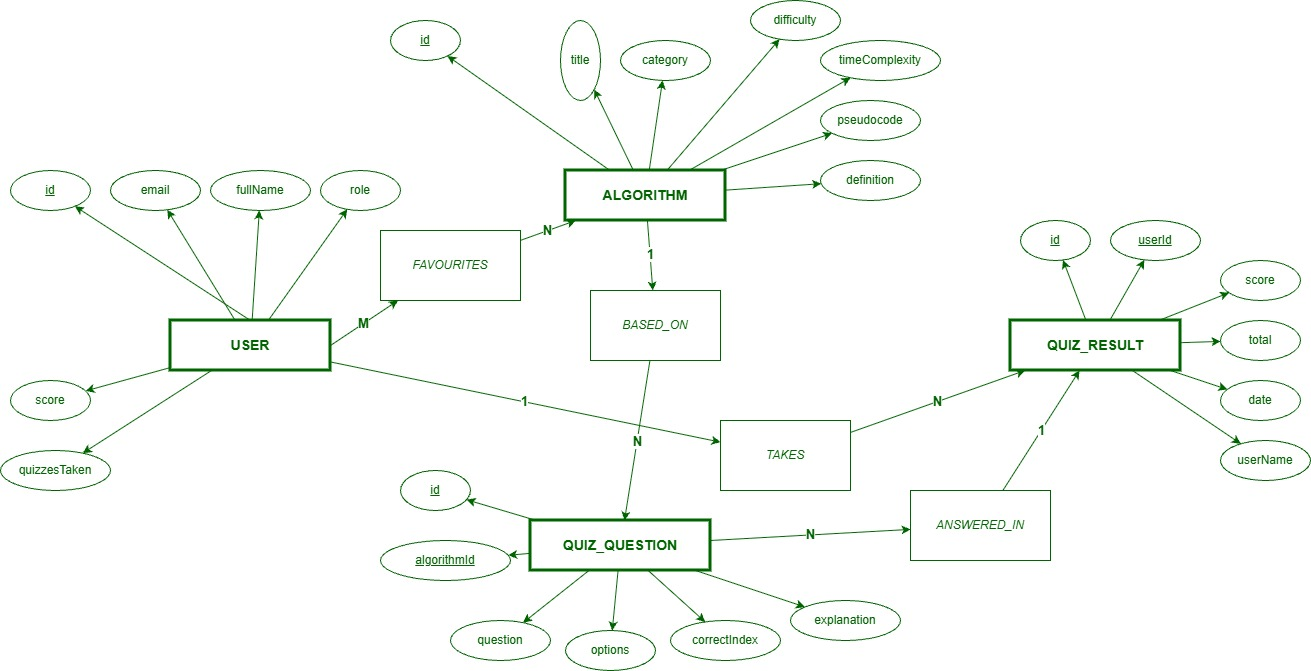
\includegraphics[width=0.90\textwidth]{SS/ER_Diagram.jpeg}
  \caption*{Figure-2: ER Diagram of AlgoFlash App}
\end{figure}

% ══════════════════════════════════════════════════════════════════════════════
\section*{Sequence Diagram --- Login Flow}
% ══════════════════════════════════════════════════════════════════════════════

\begin{figure}[H]
  \centering
  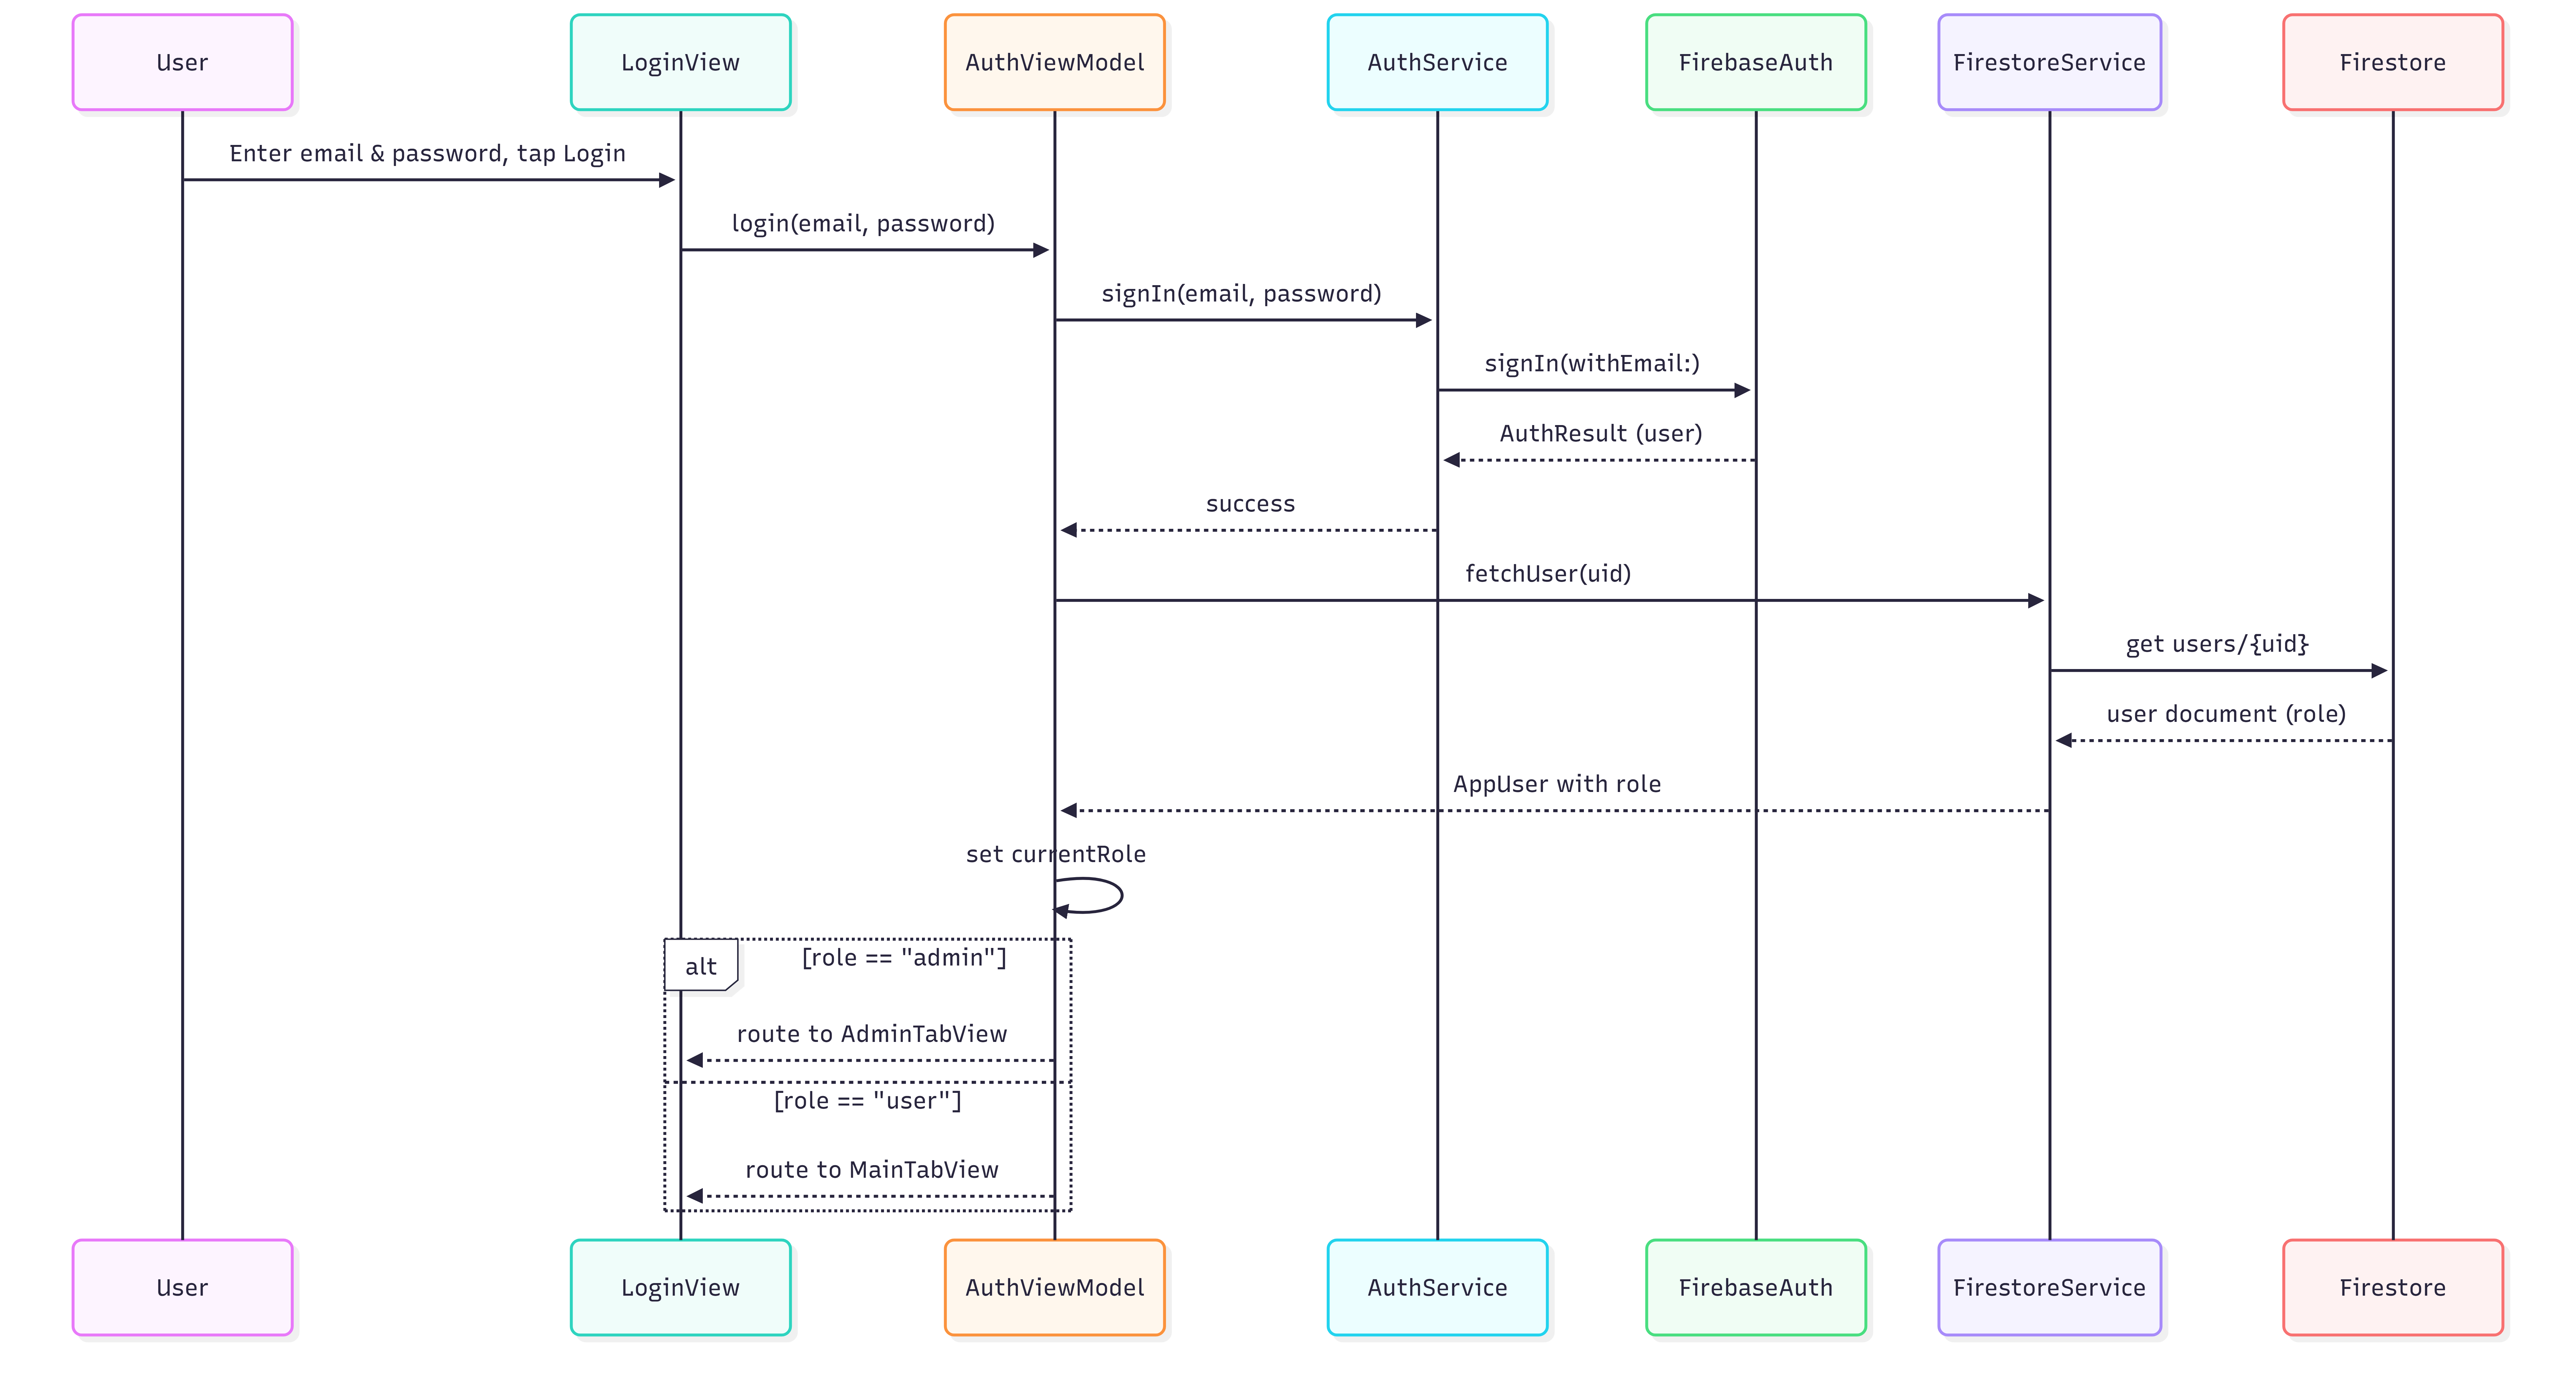
\includegraphics[width=\textwidth]{SS/sequence.png}
  \caption*{Figure-3: Login Sequence Diagram of AlgoFlash App}
\end{figure}

\newpage
% ══════════════════════════════════════════════════════════════════════════════
\section*{Application Screenshots}
% ══════════════════════════════════════════════════════════════════════════════

All screenshots were captured on iPhone 17 Pro running iOS 26.4 using the iOS Simulator.

\begin{figure}[H]
  \centering
  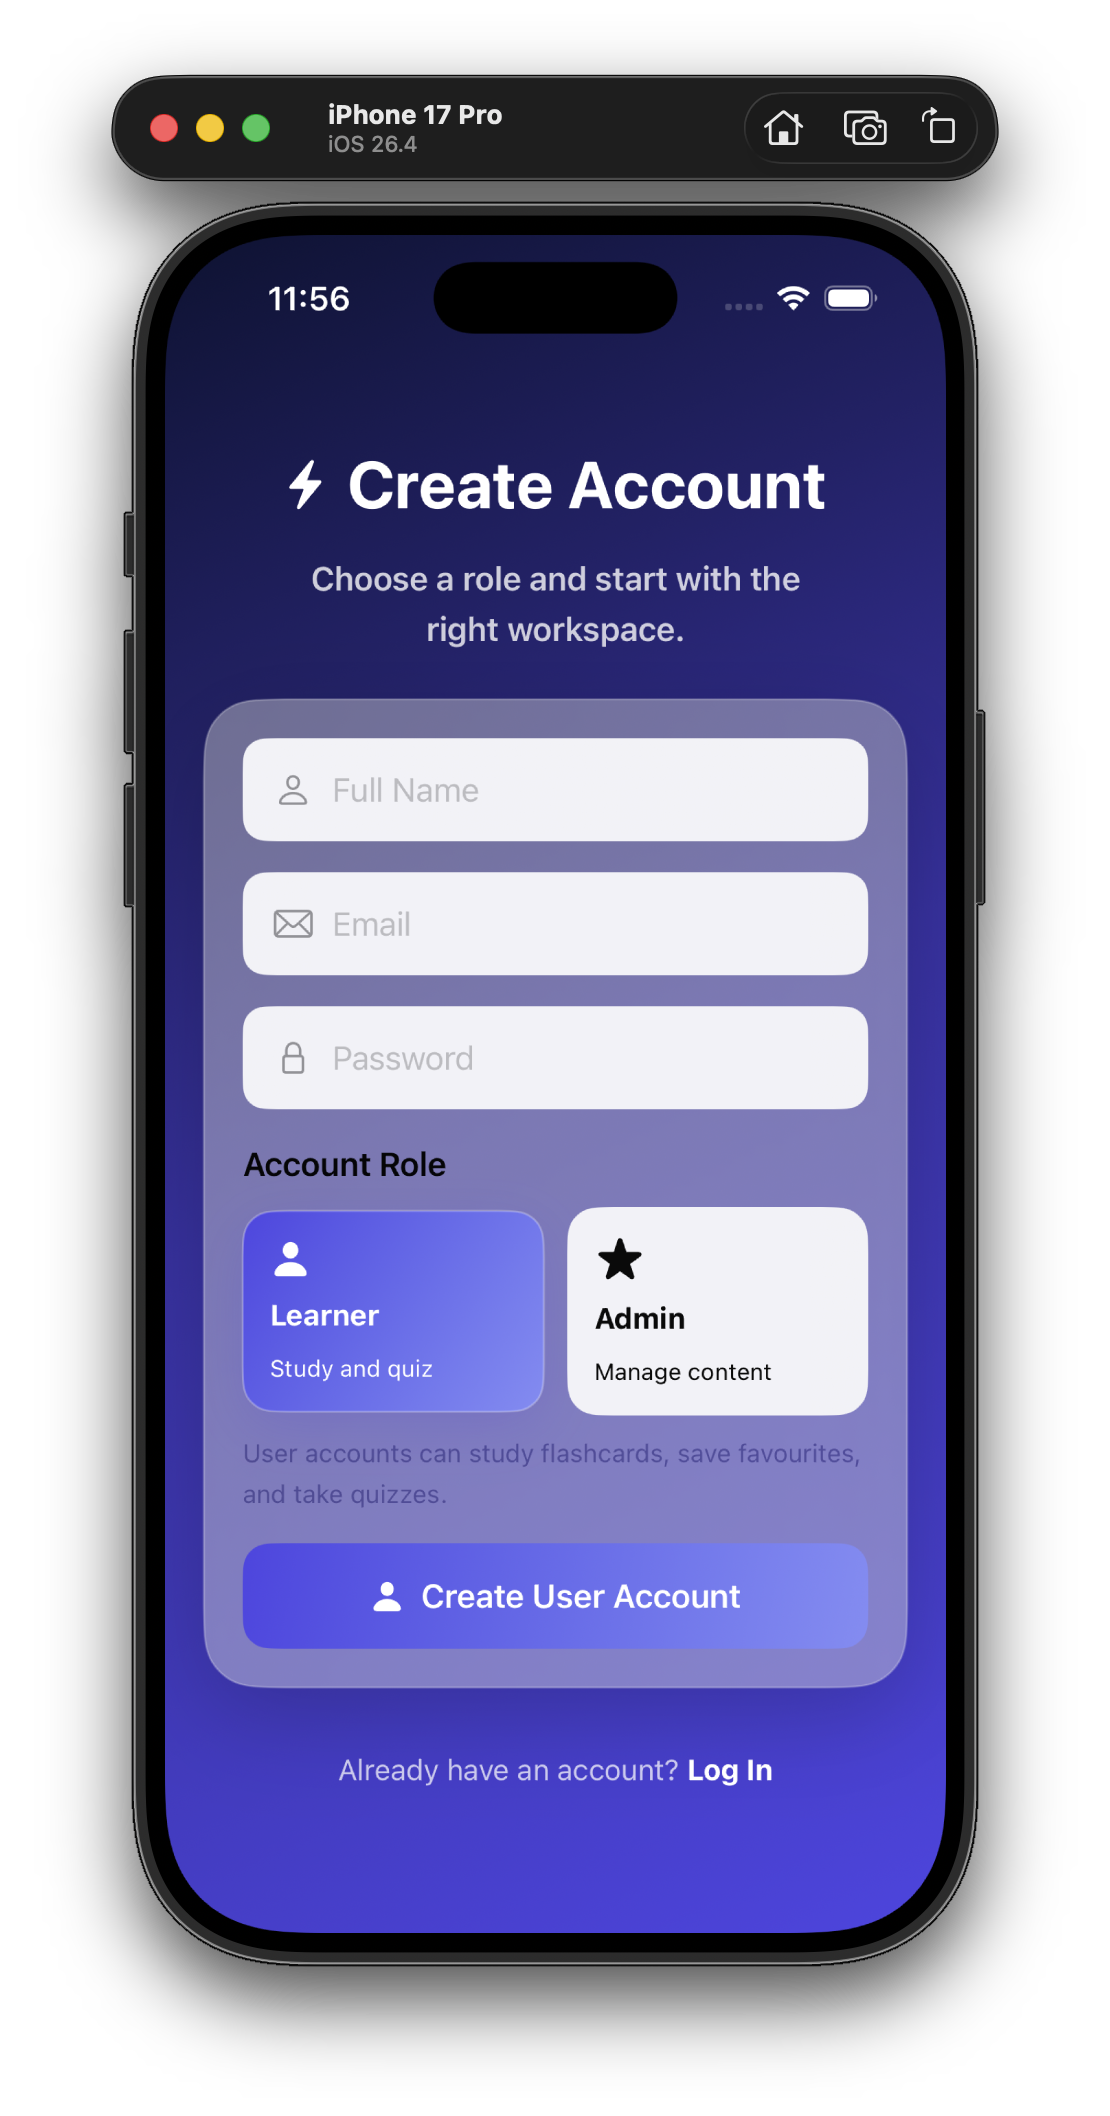
\includegraphics[width=0.30\textwidth]{SS/1. sign_up.png}\hfill
  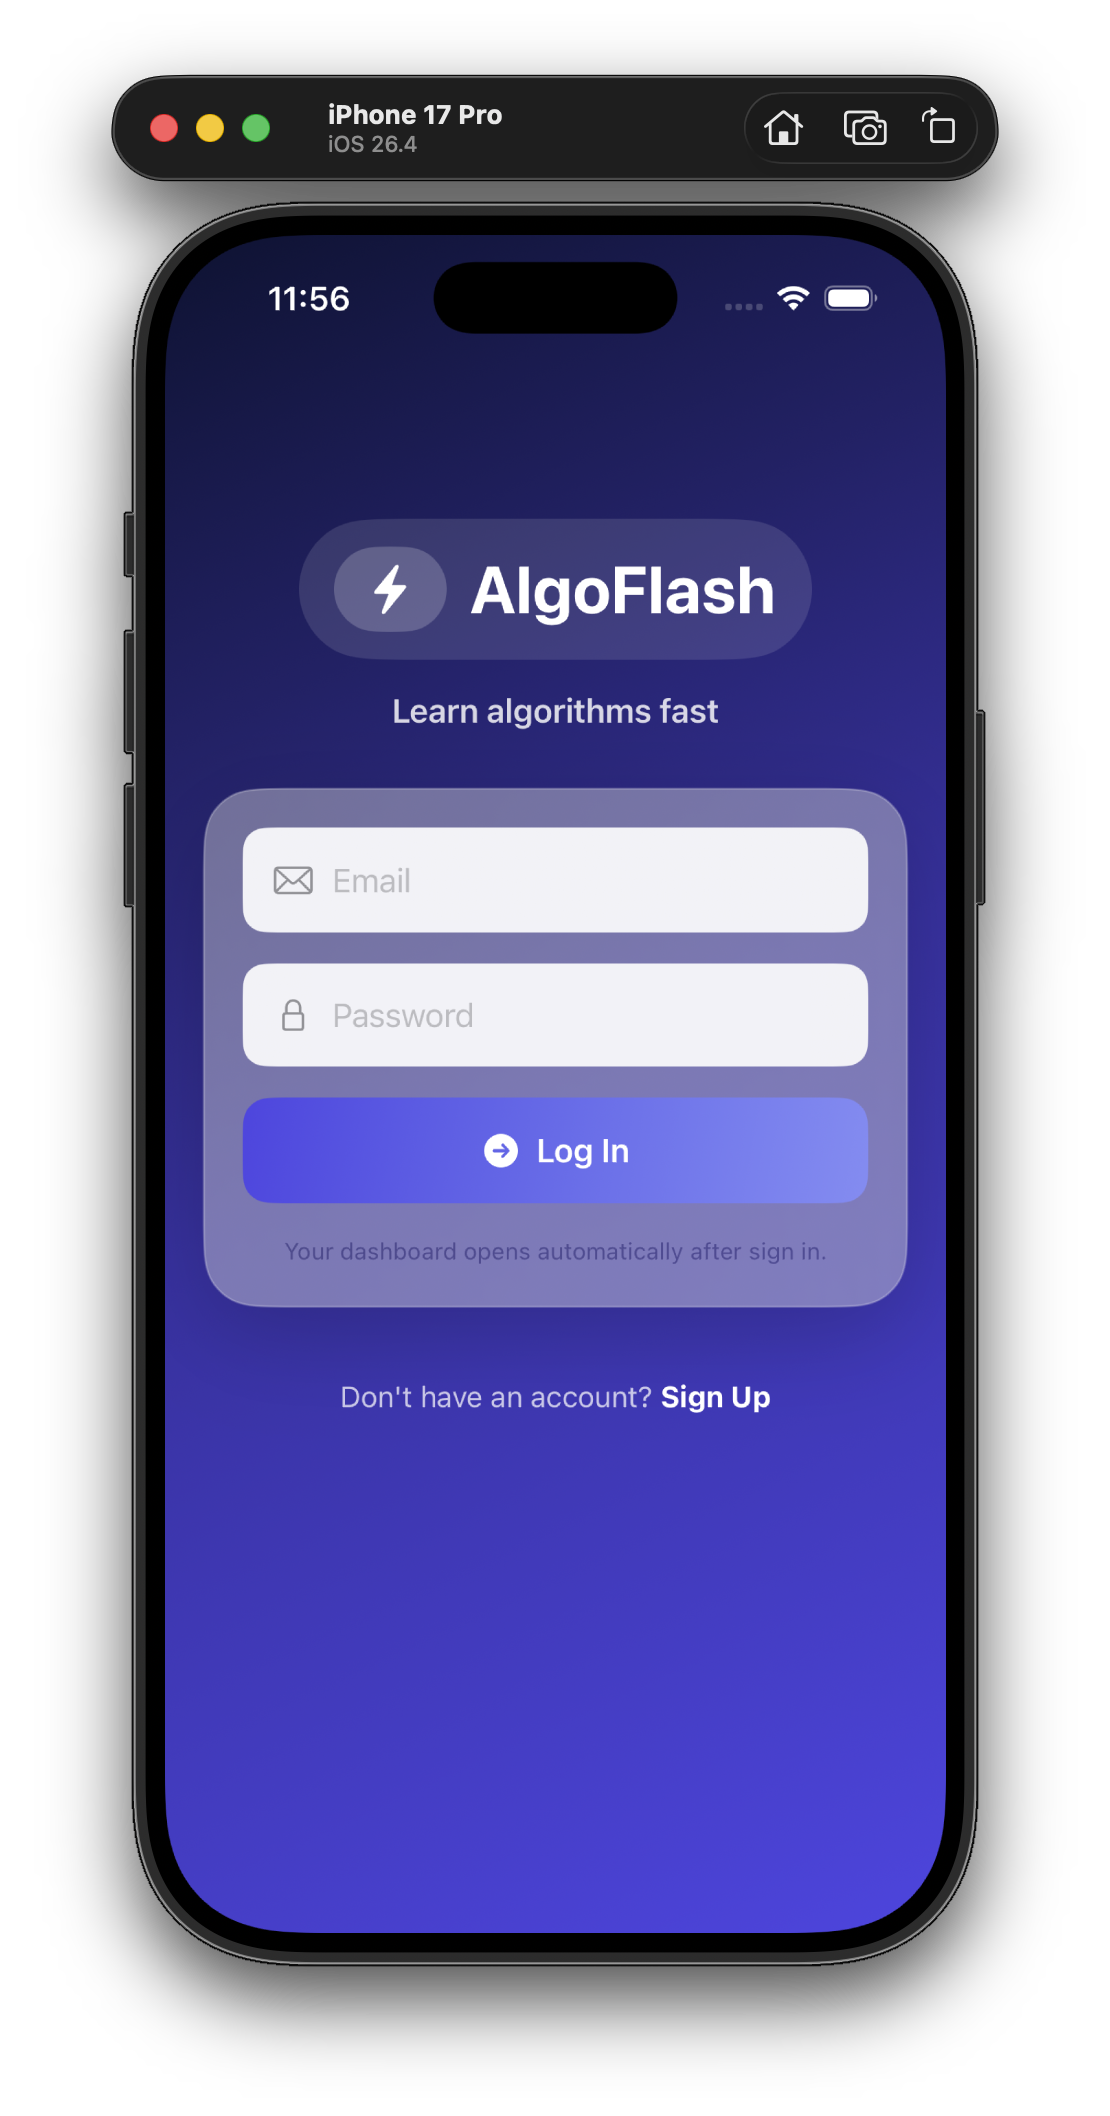
\includegraphics[width=0.30\textwidth]{SS/2. login.png}\hfill
  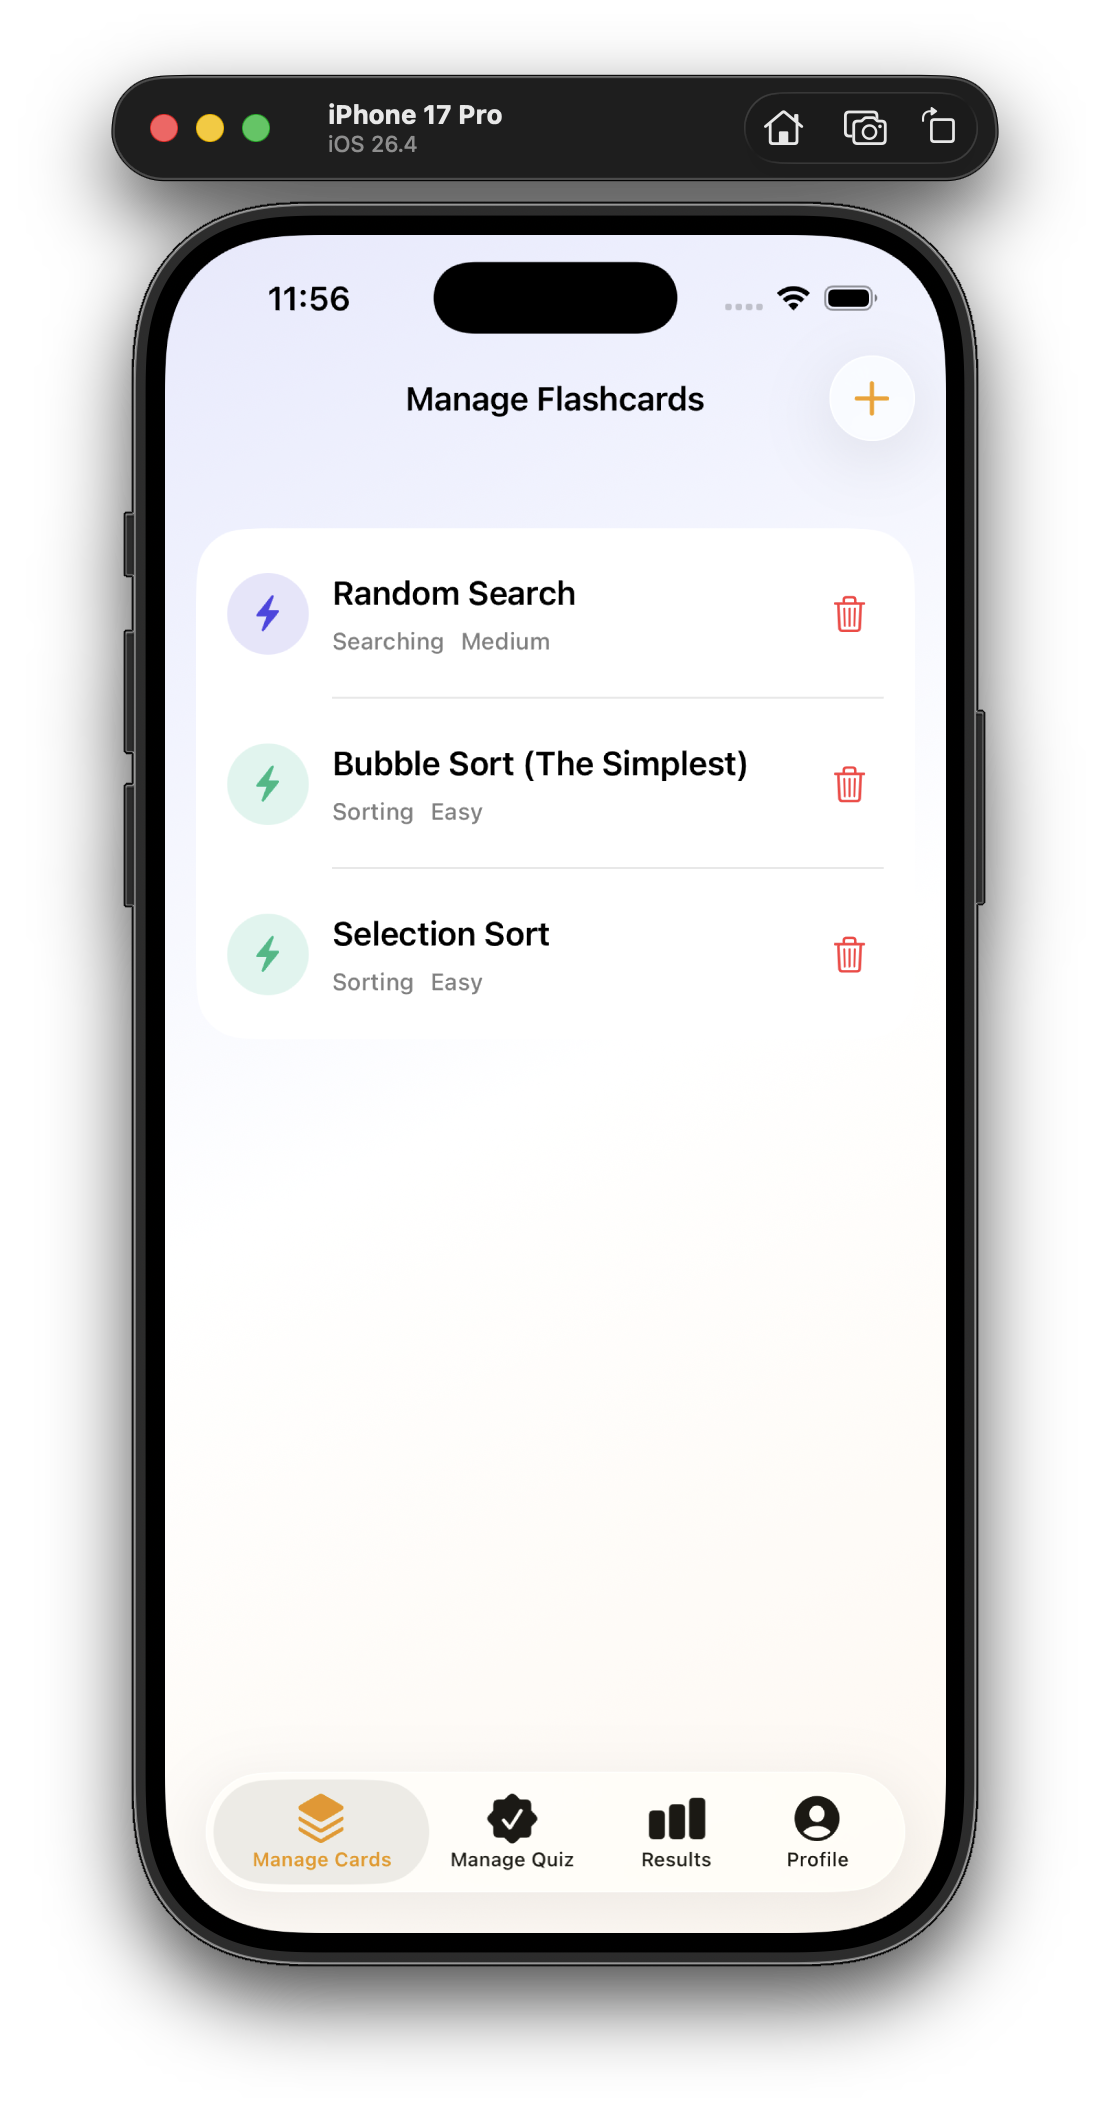
\includegraphics[width=0.30\textwidth]{SS/3. admin_manage_flashcard.png}\\[0.8em]
  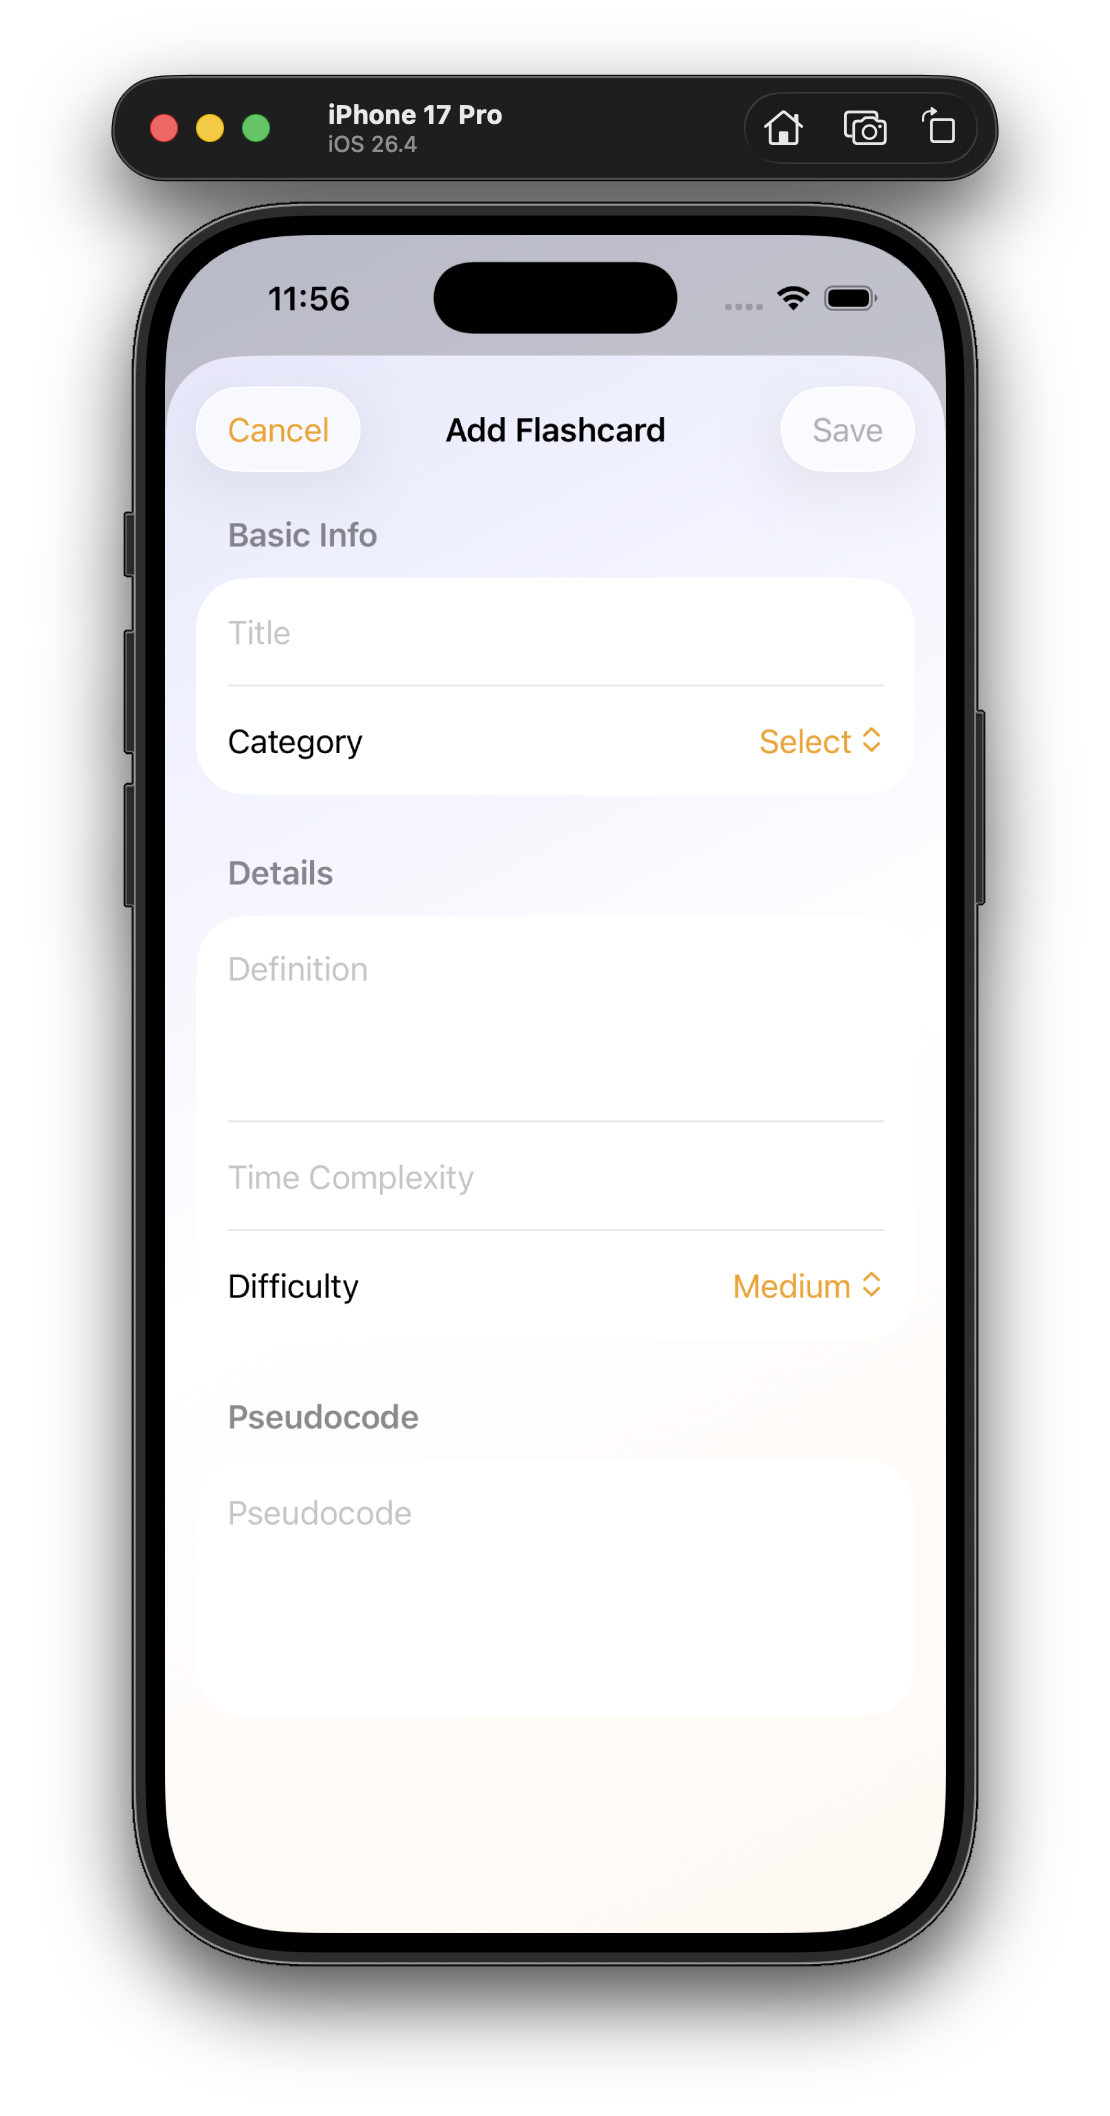
\includegraphics[width=0.30\textwidth]{SS/4. admin_flashcard_add_modal.png}\hfill
  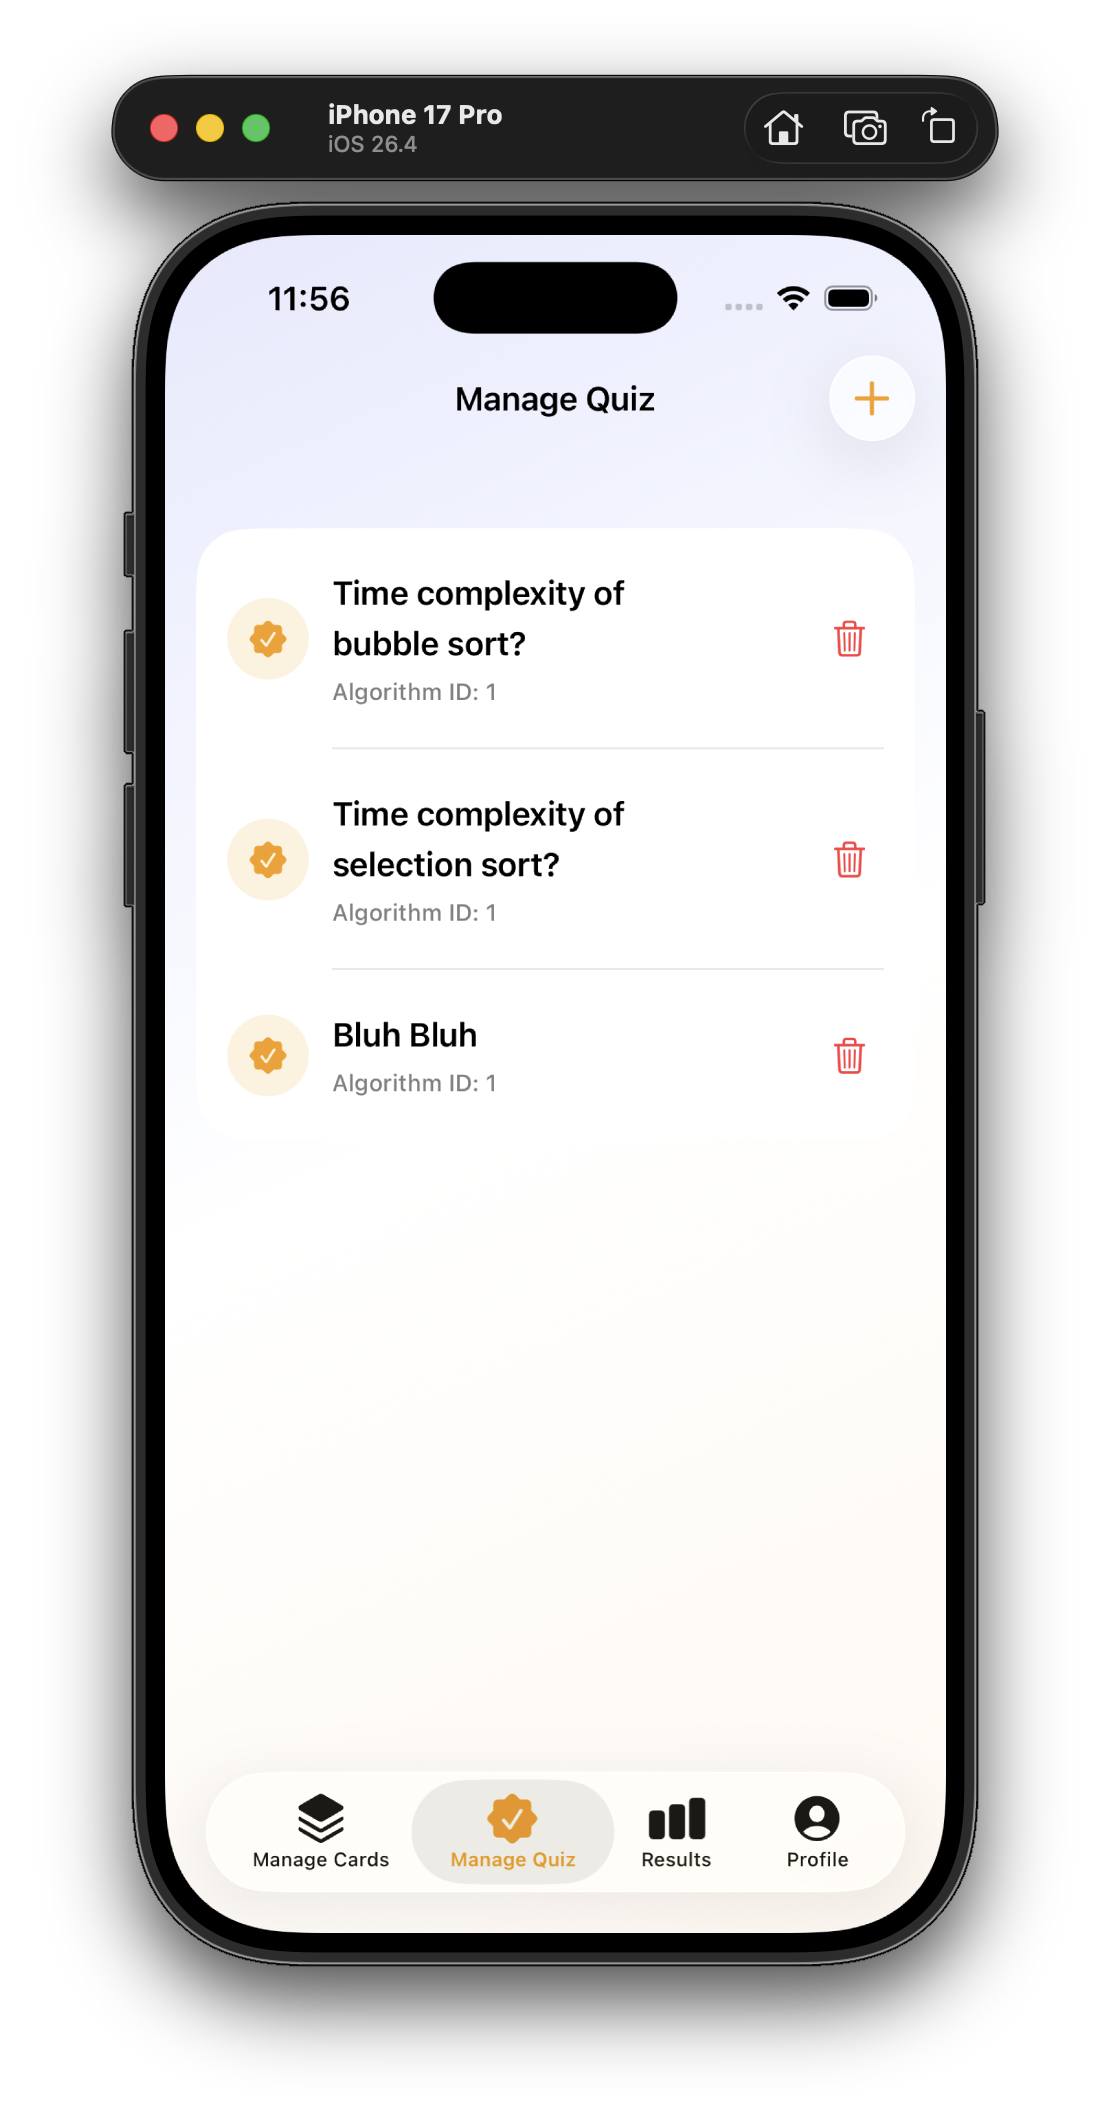
\includegraphics[width=0.30\textwidth]{SS/5. admin_manage_quizz.png}\hfill
  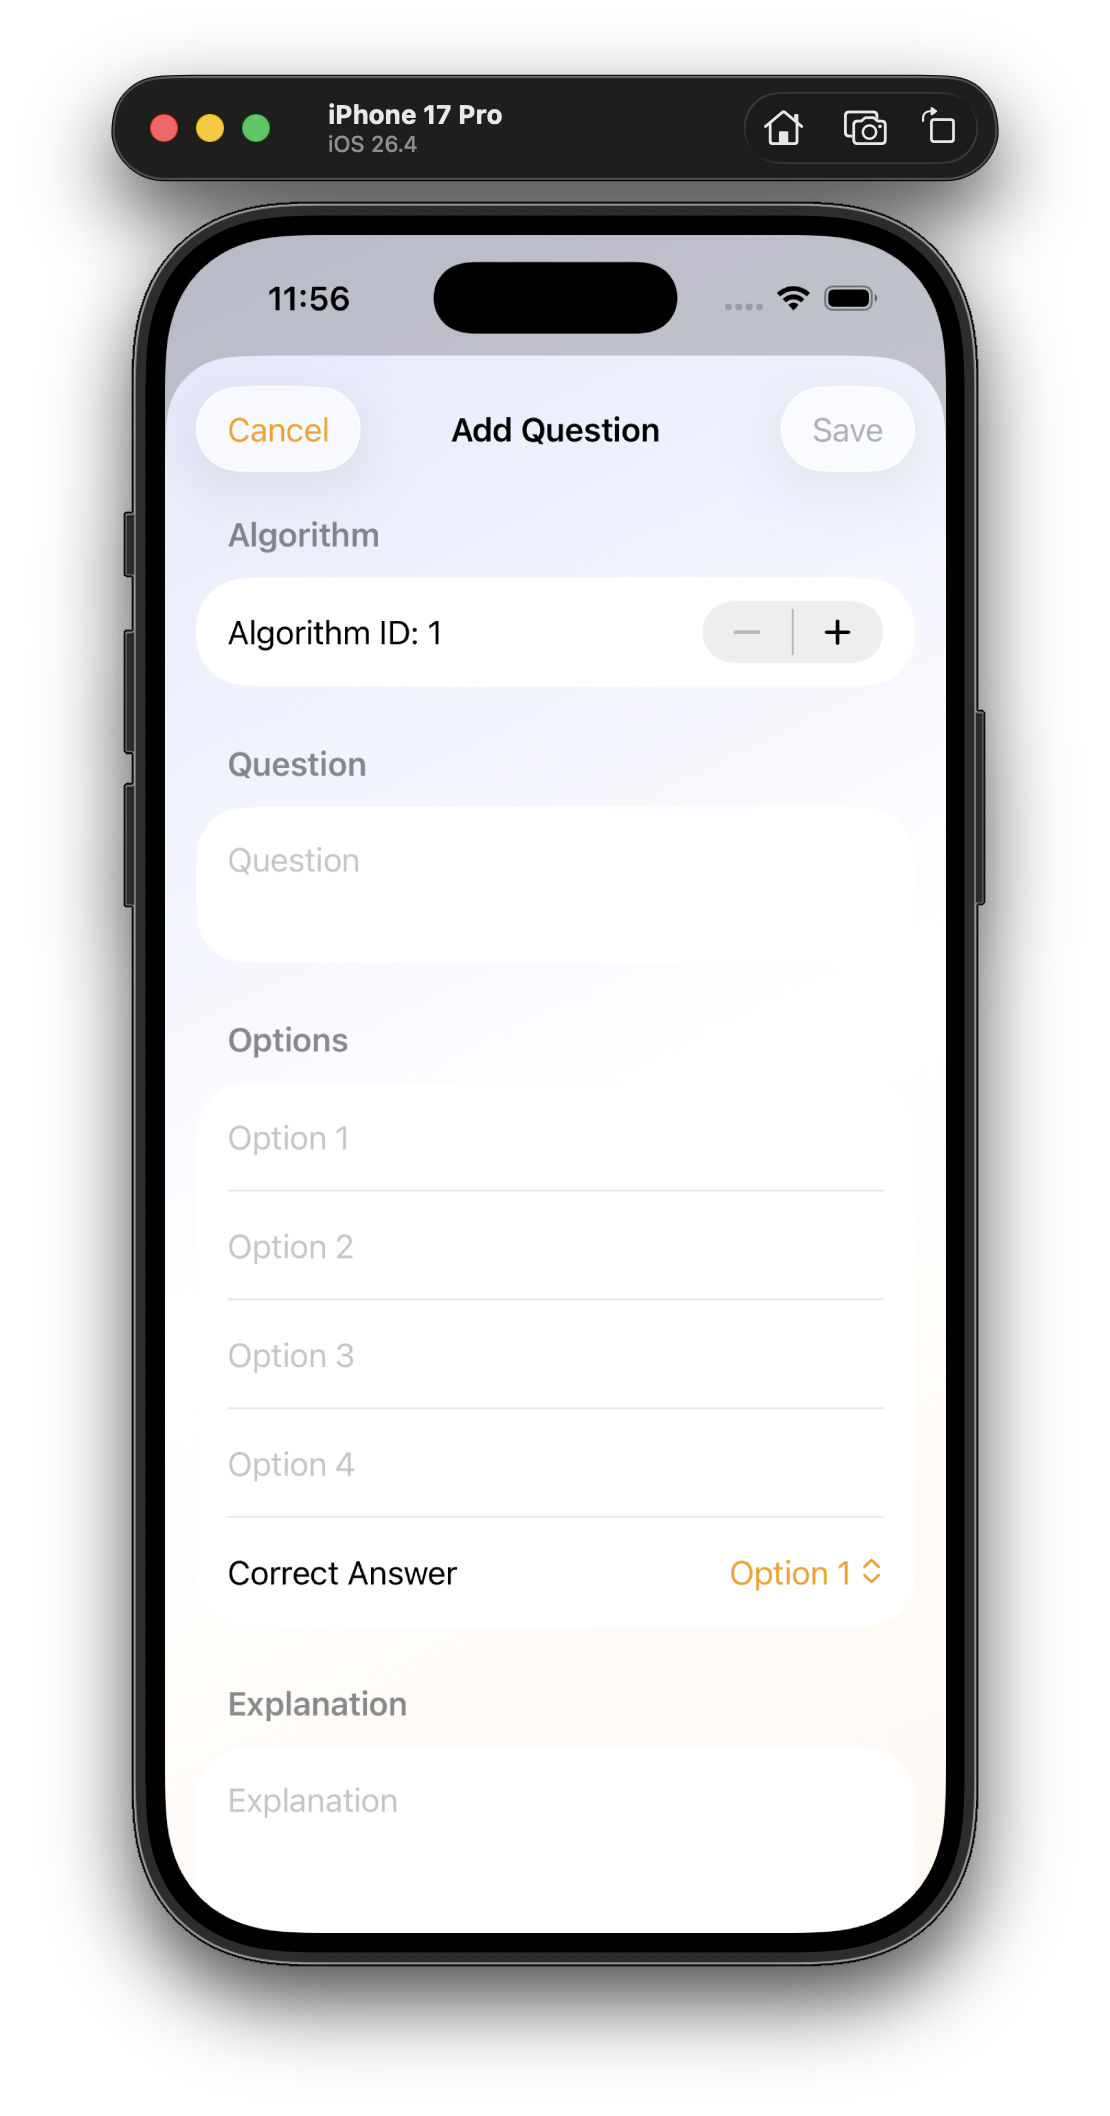
\includegraphics[width=0.30\textwidth]{SS/6. admin_add_quiz_modal.png}
  \caption*{Figure-4: Authentication and Admin Content Management Screens}
\end{figure}

\begin{figure}[H]
  \centering
  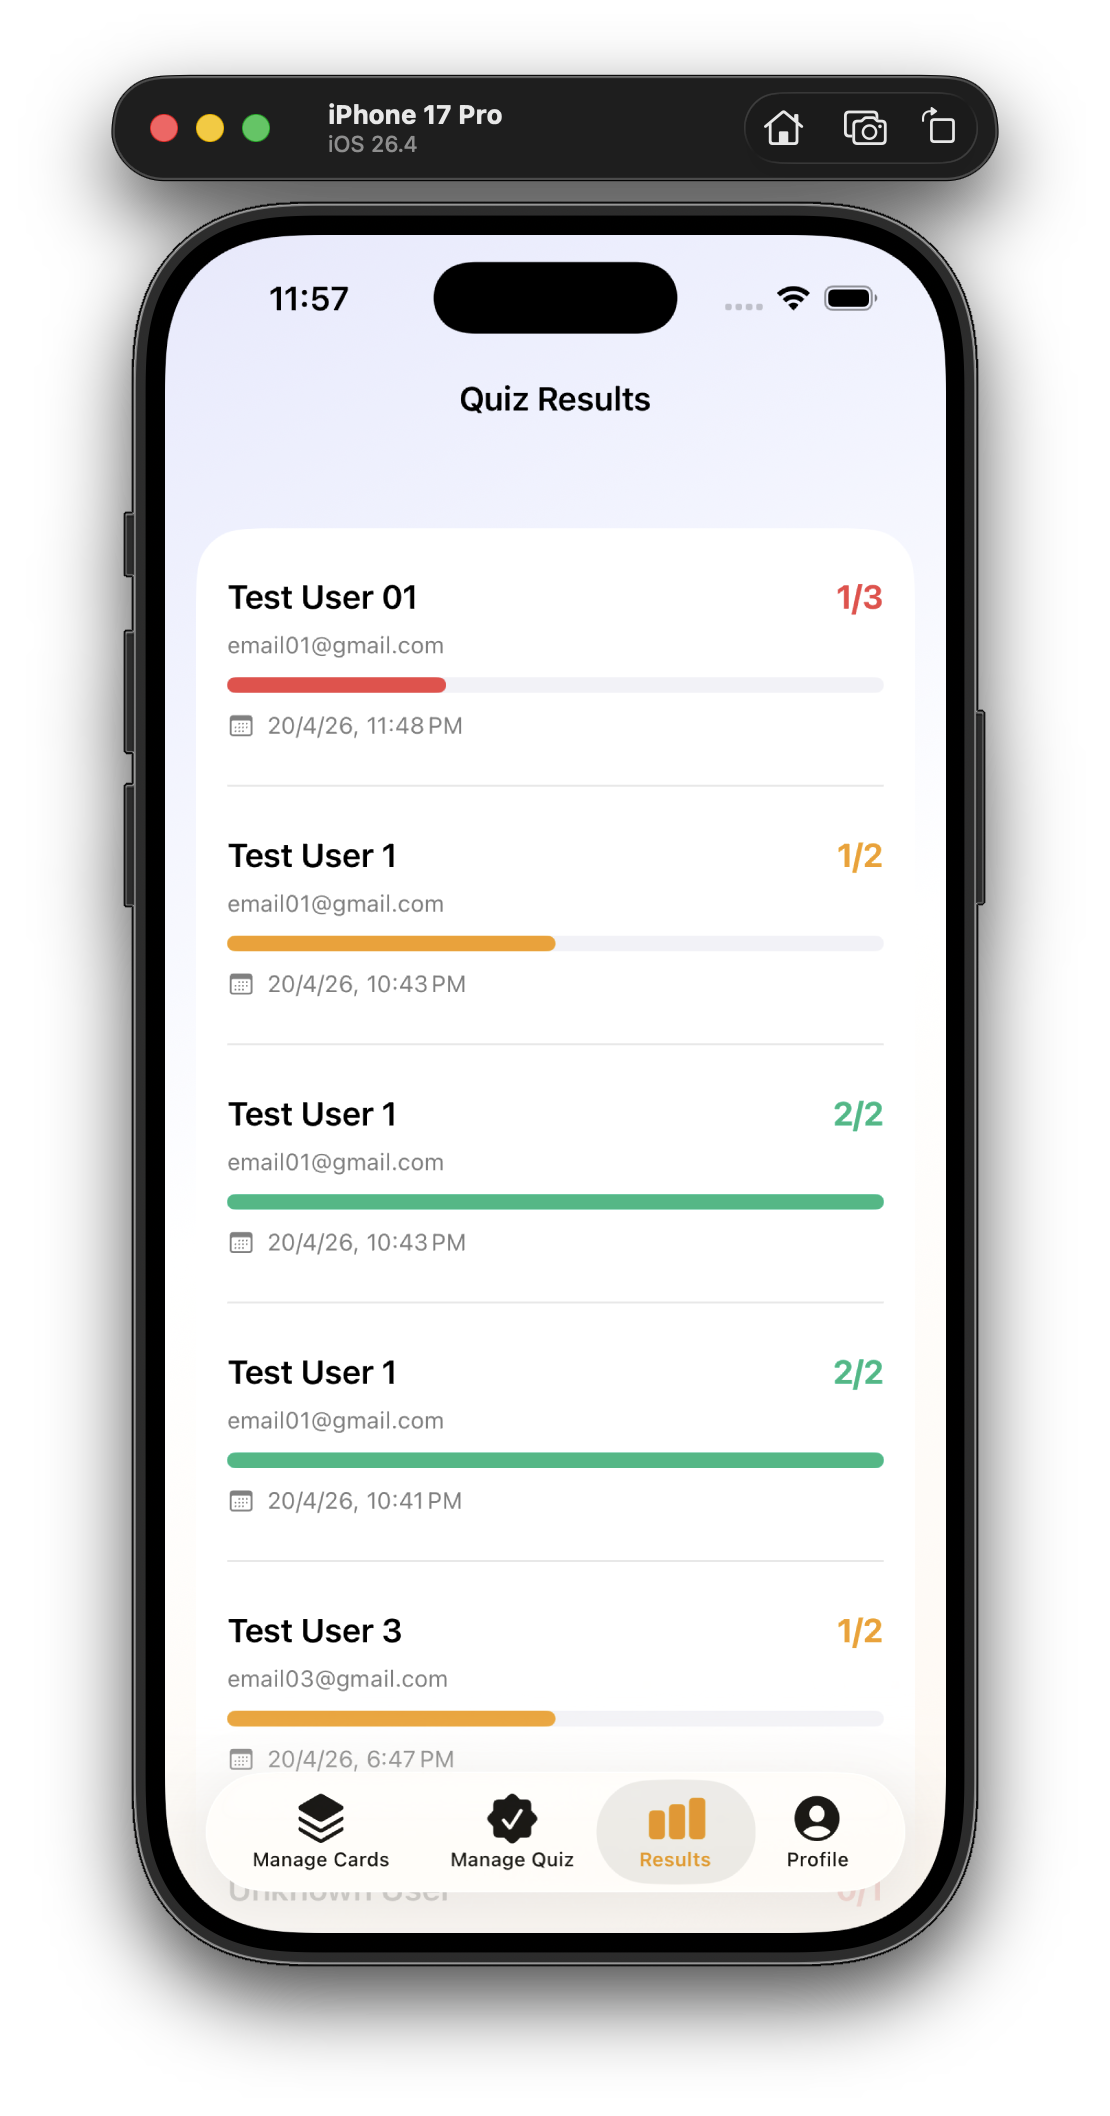
\includegraphics[width=0.30\textwidth]{SS/7. admin_results.png}\hfill
  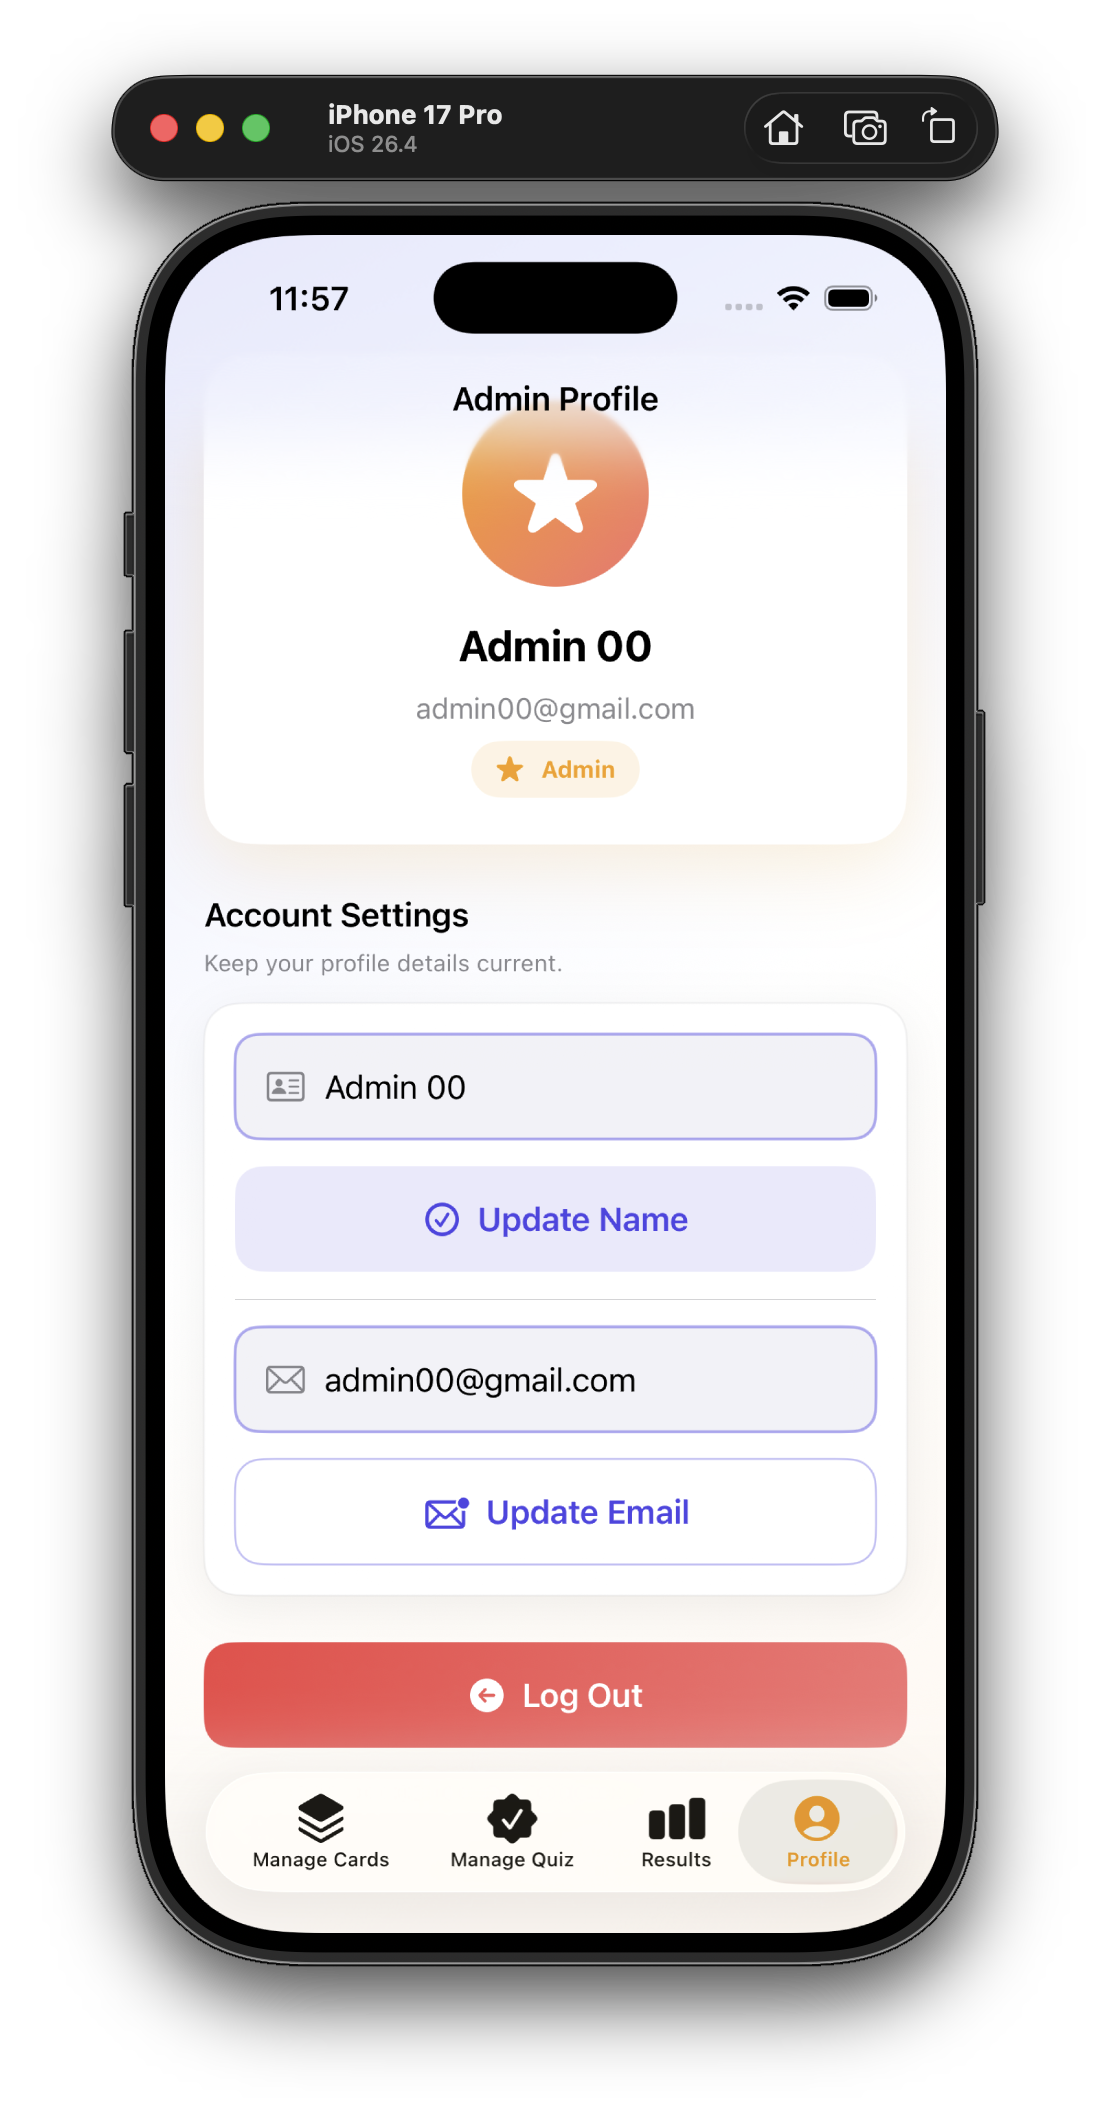
\includegraphics[width=0.30\textwidth]{SS/9. admin_profile.png}\hfill
  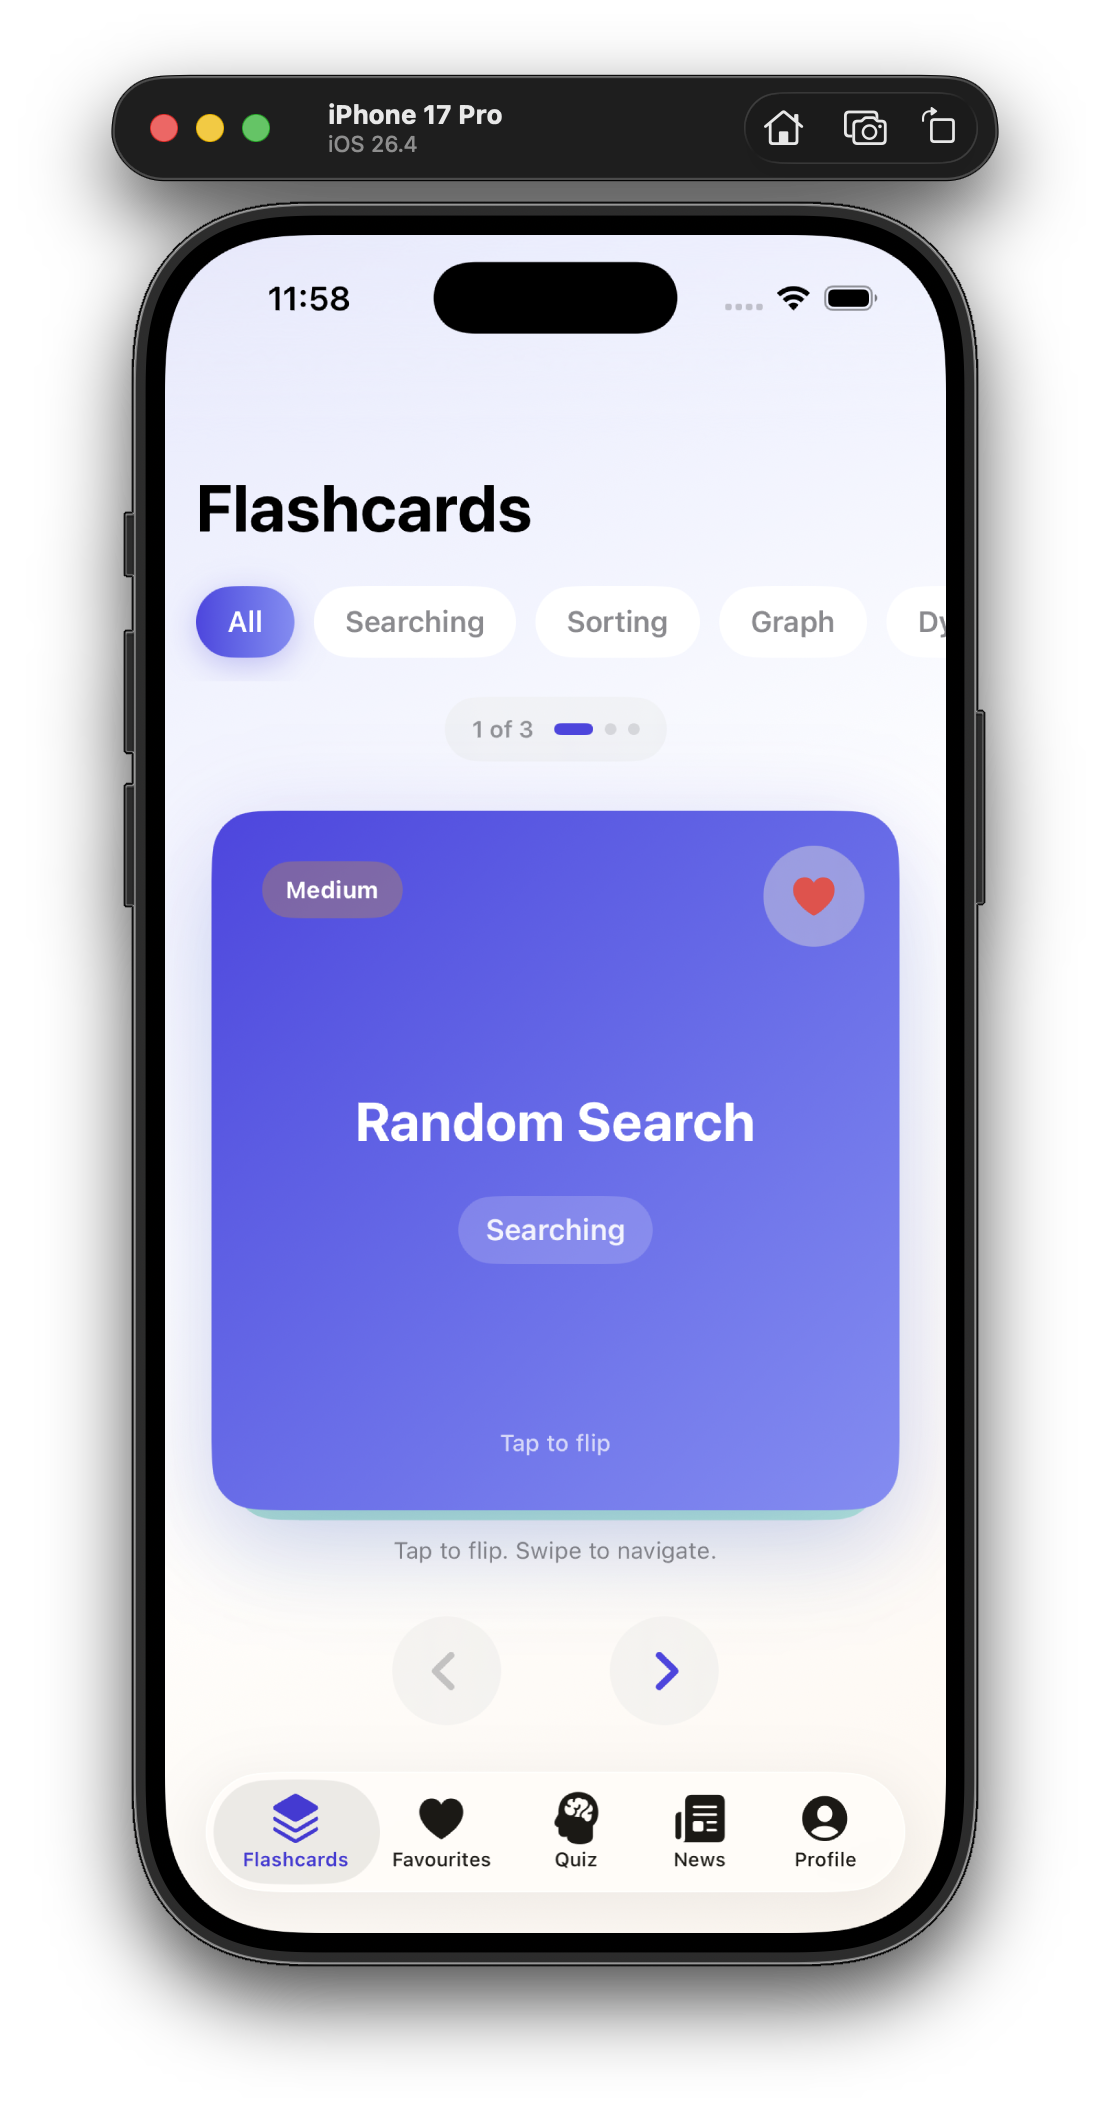
\includegraphics[width=0.30\textwidth]{SS/10. user_flashcard.png}\\[0.8em]
  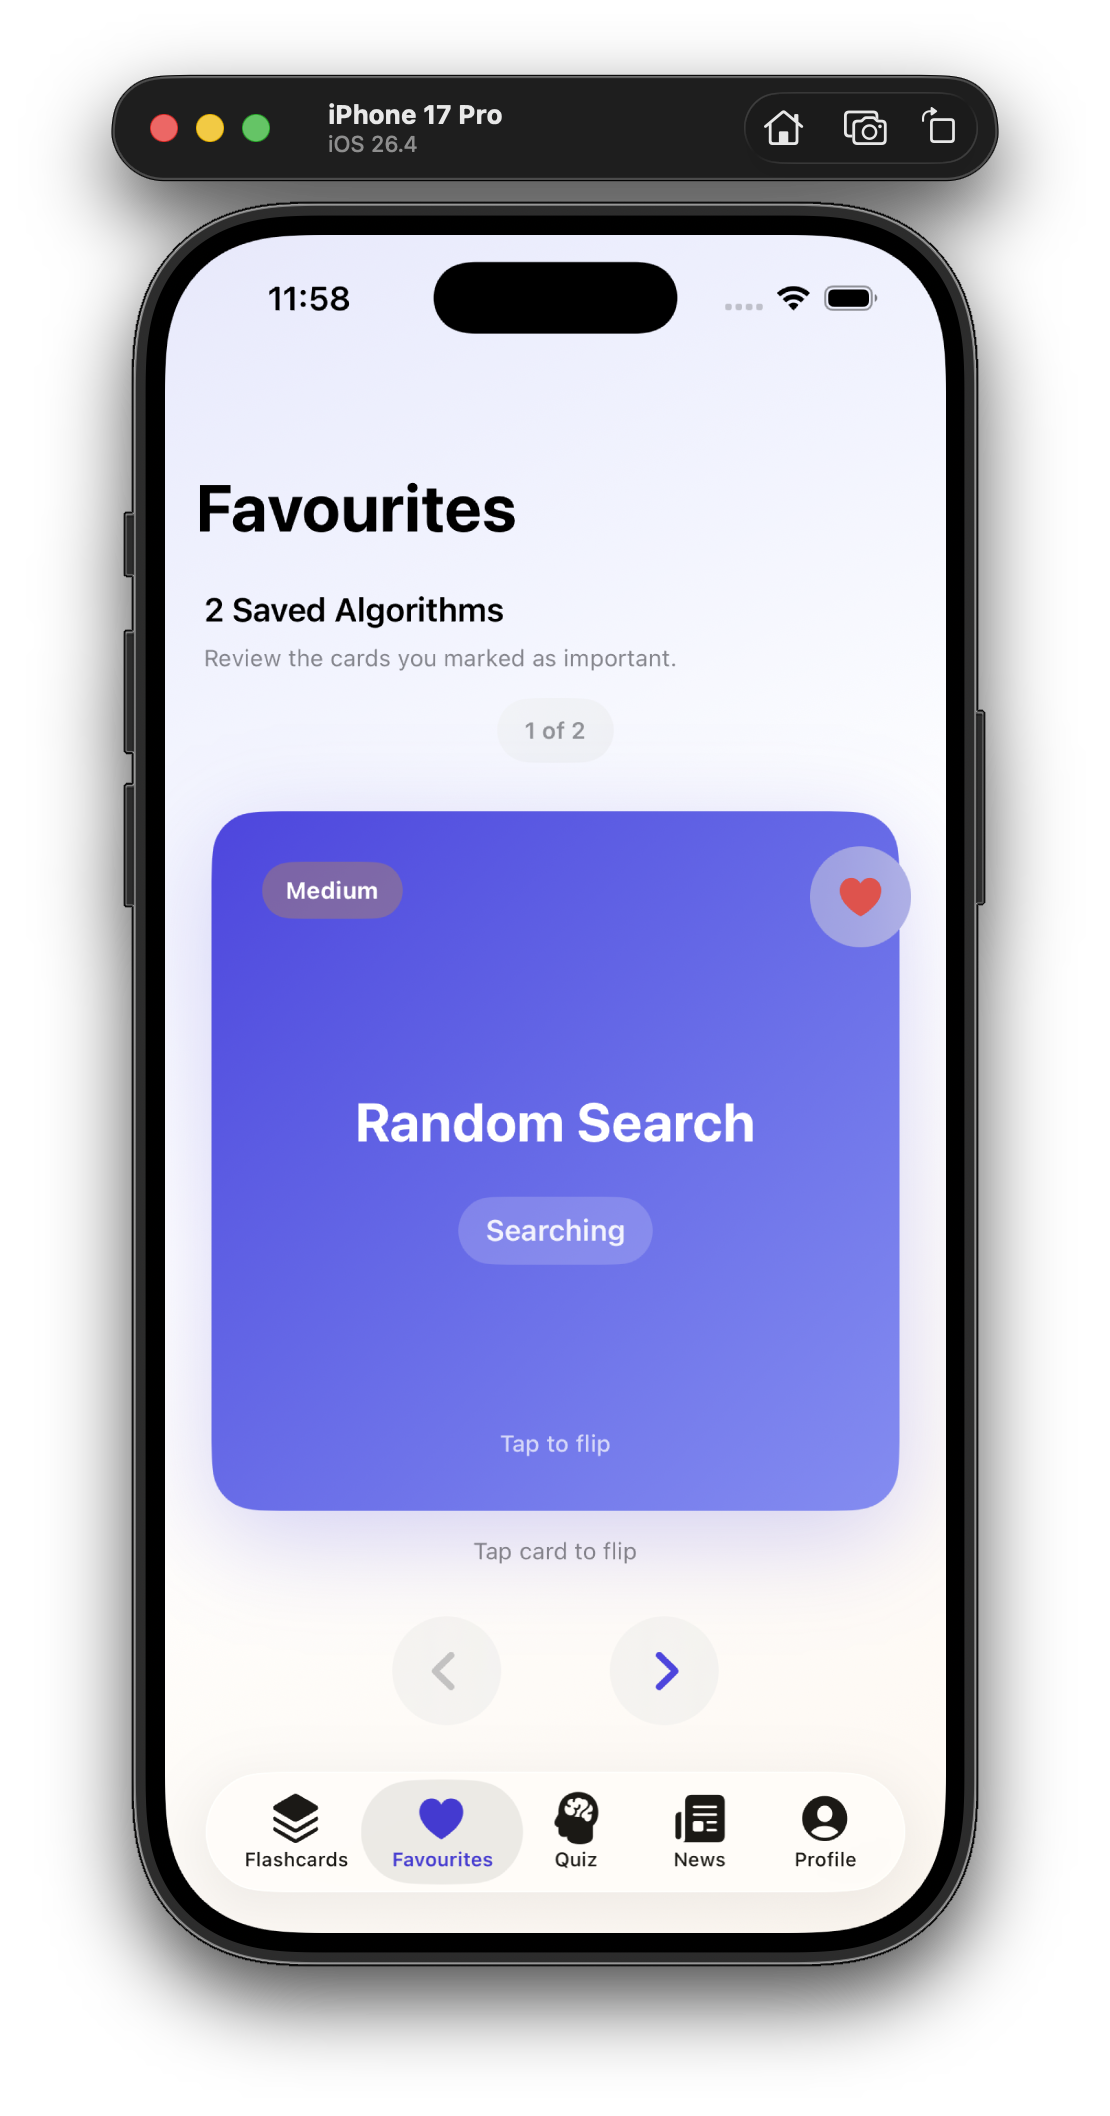
\includegraphics[width=0.30\textwidth]{SS/11. user_favourites.png}\hfill
  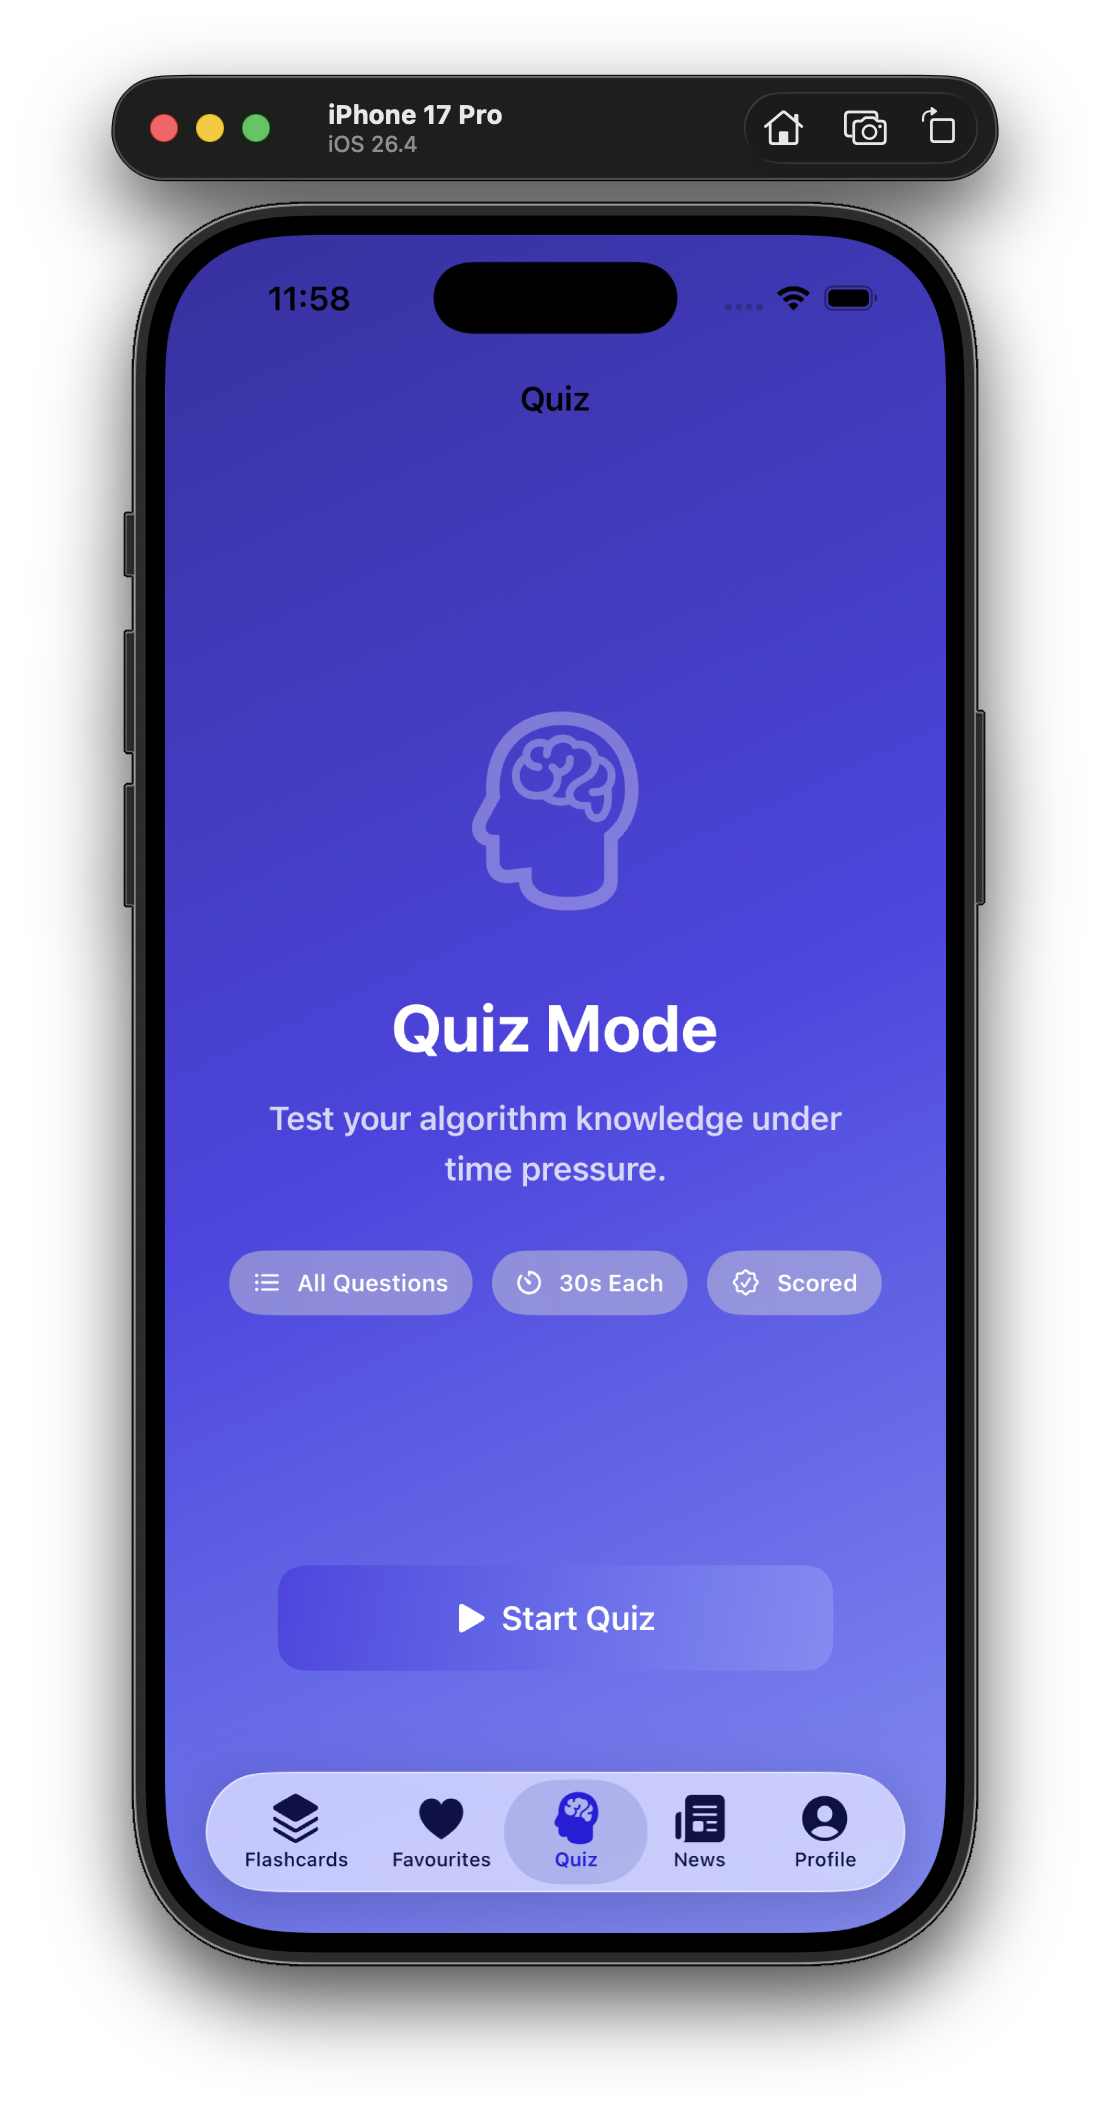
\includegraphics[width=0.30\textwidth]{SS/12. user_quiz.png}\hfill
  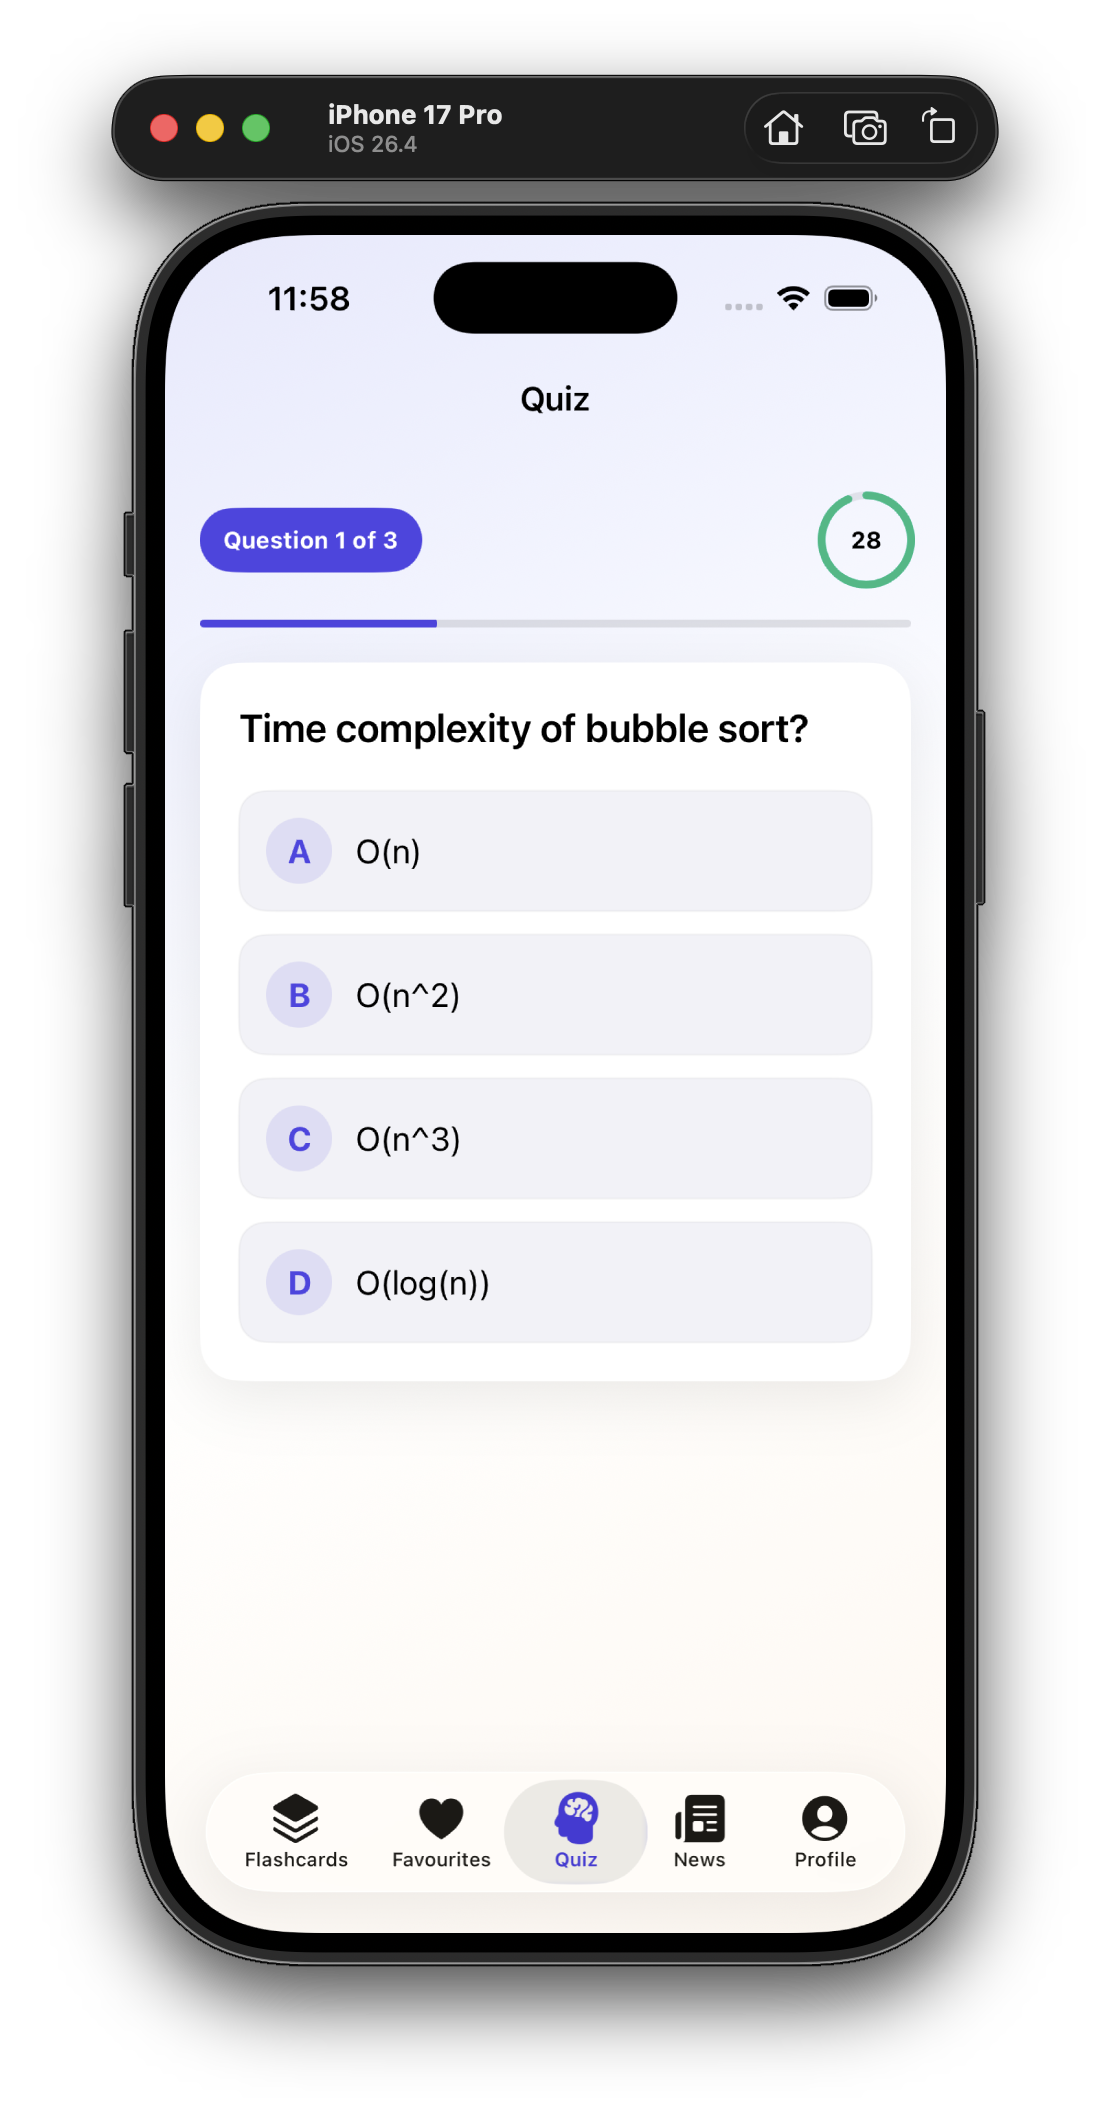
\includegraphics[width=0.30\textwidth]{SS/13. user_participating_quiz.png}
  \caption*{Figure-5: Admin Results \& Profile, User Flashcards, Favourites, and Quiz Screens}
\end{figure}

\begin{figure}[H]
  \centering
  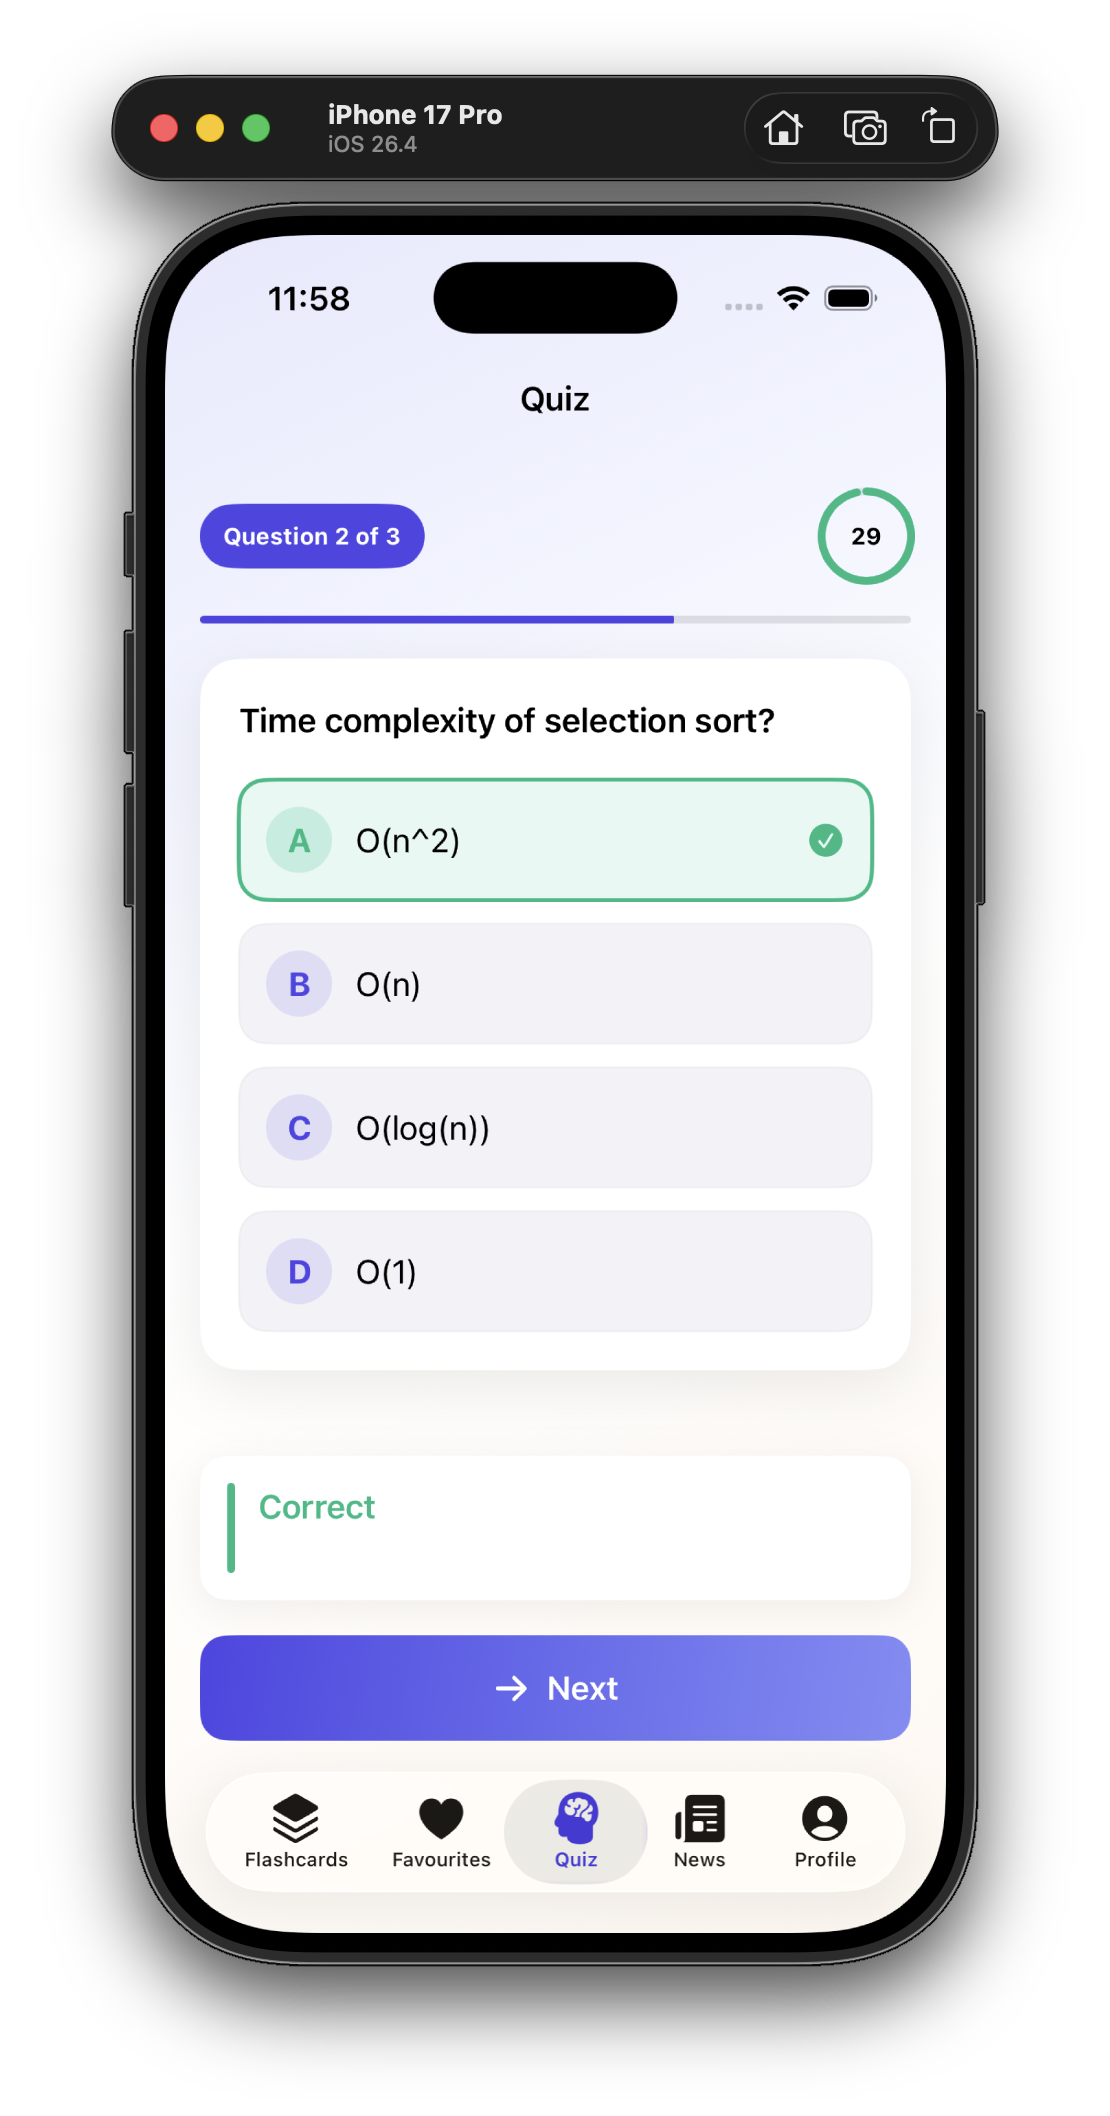
\includegraphics[width=0.30\textwidth]{SS/15. user_participating_quiz_correct_submission.png}\hfill
  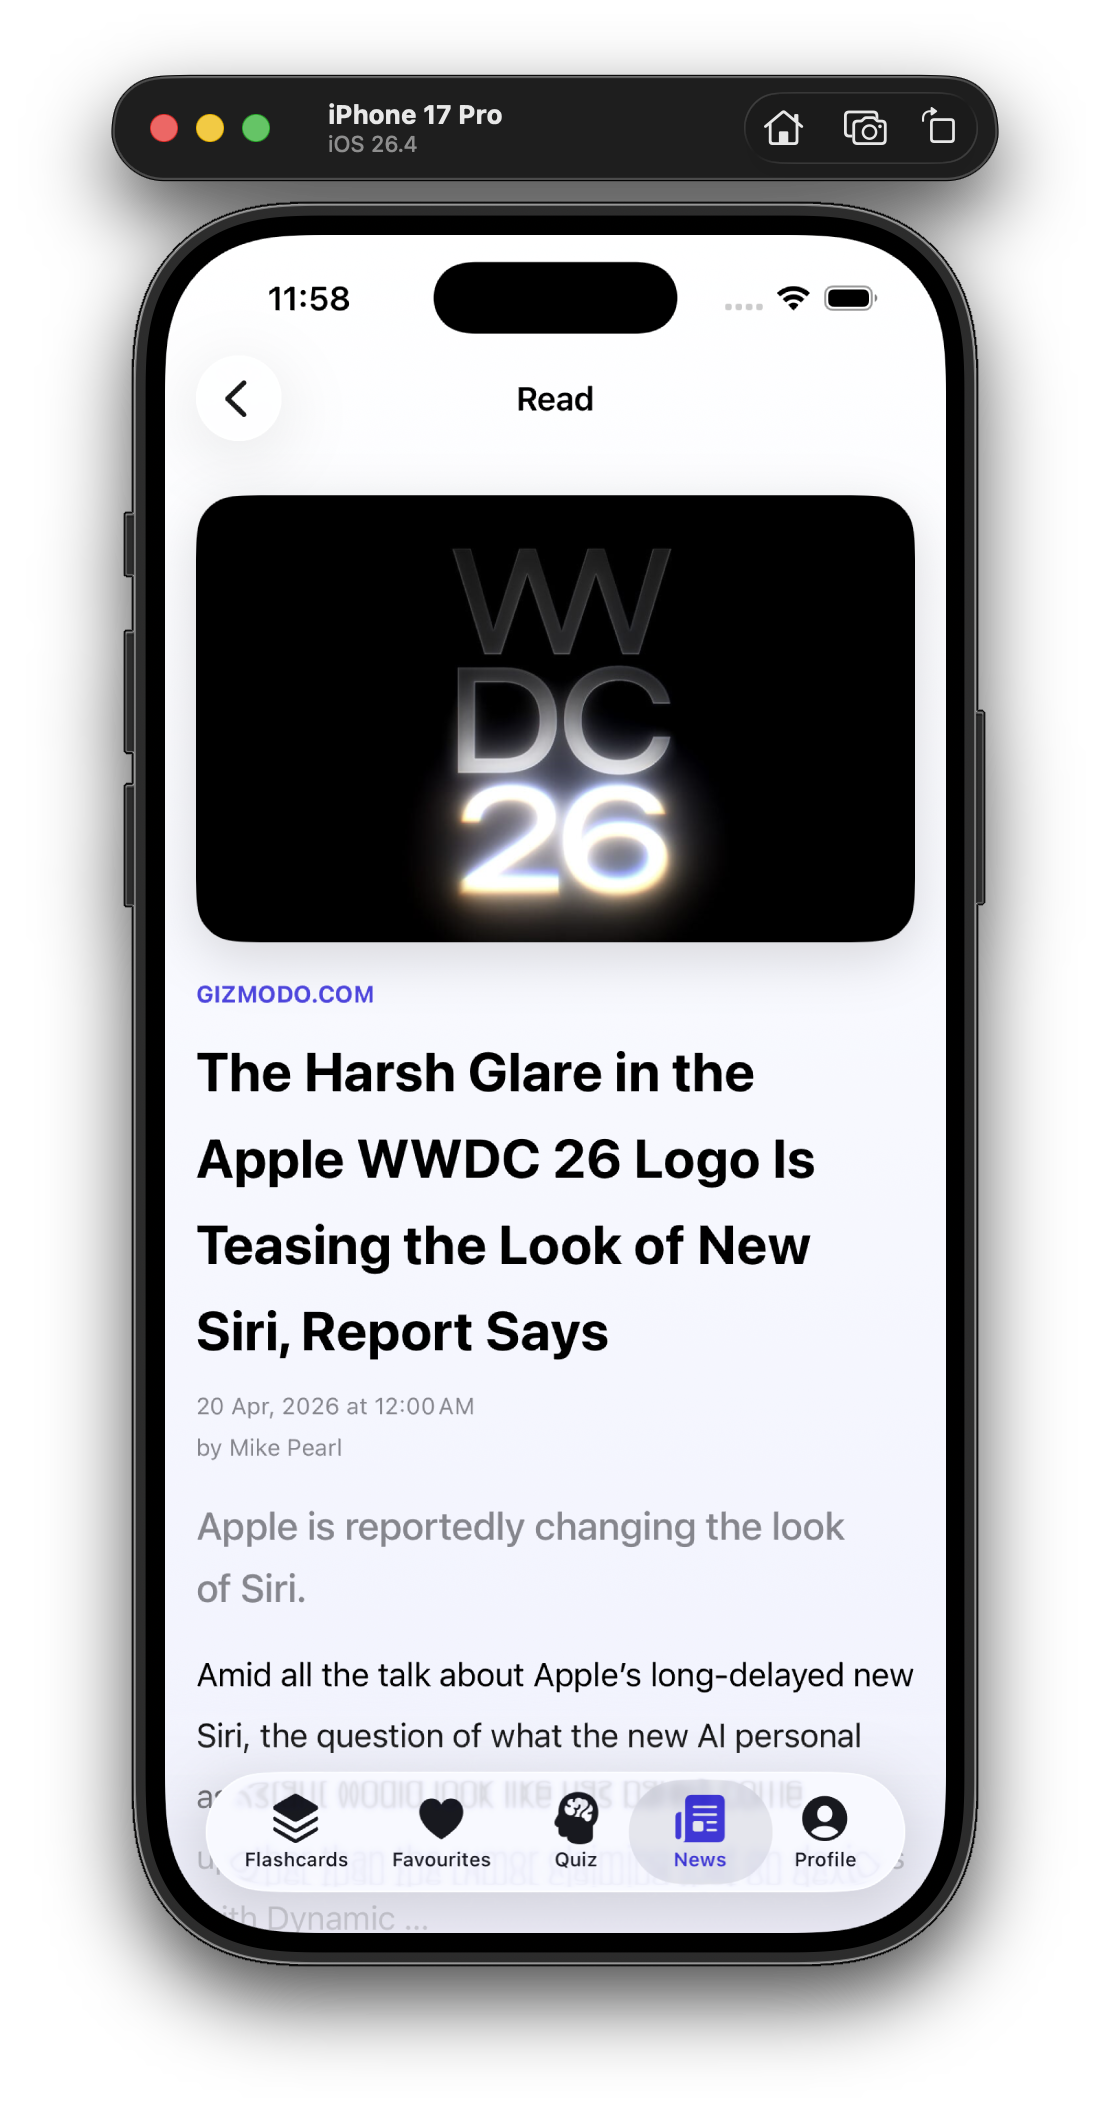
\includegraphics[width=0.30\textwidth]{SS/17. user_news_details_view.png}\hfill
  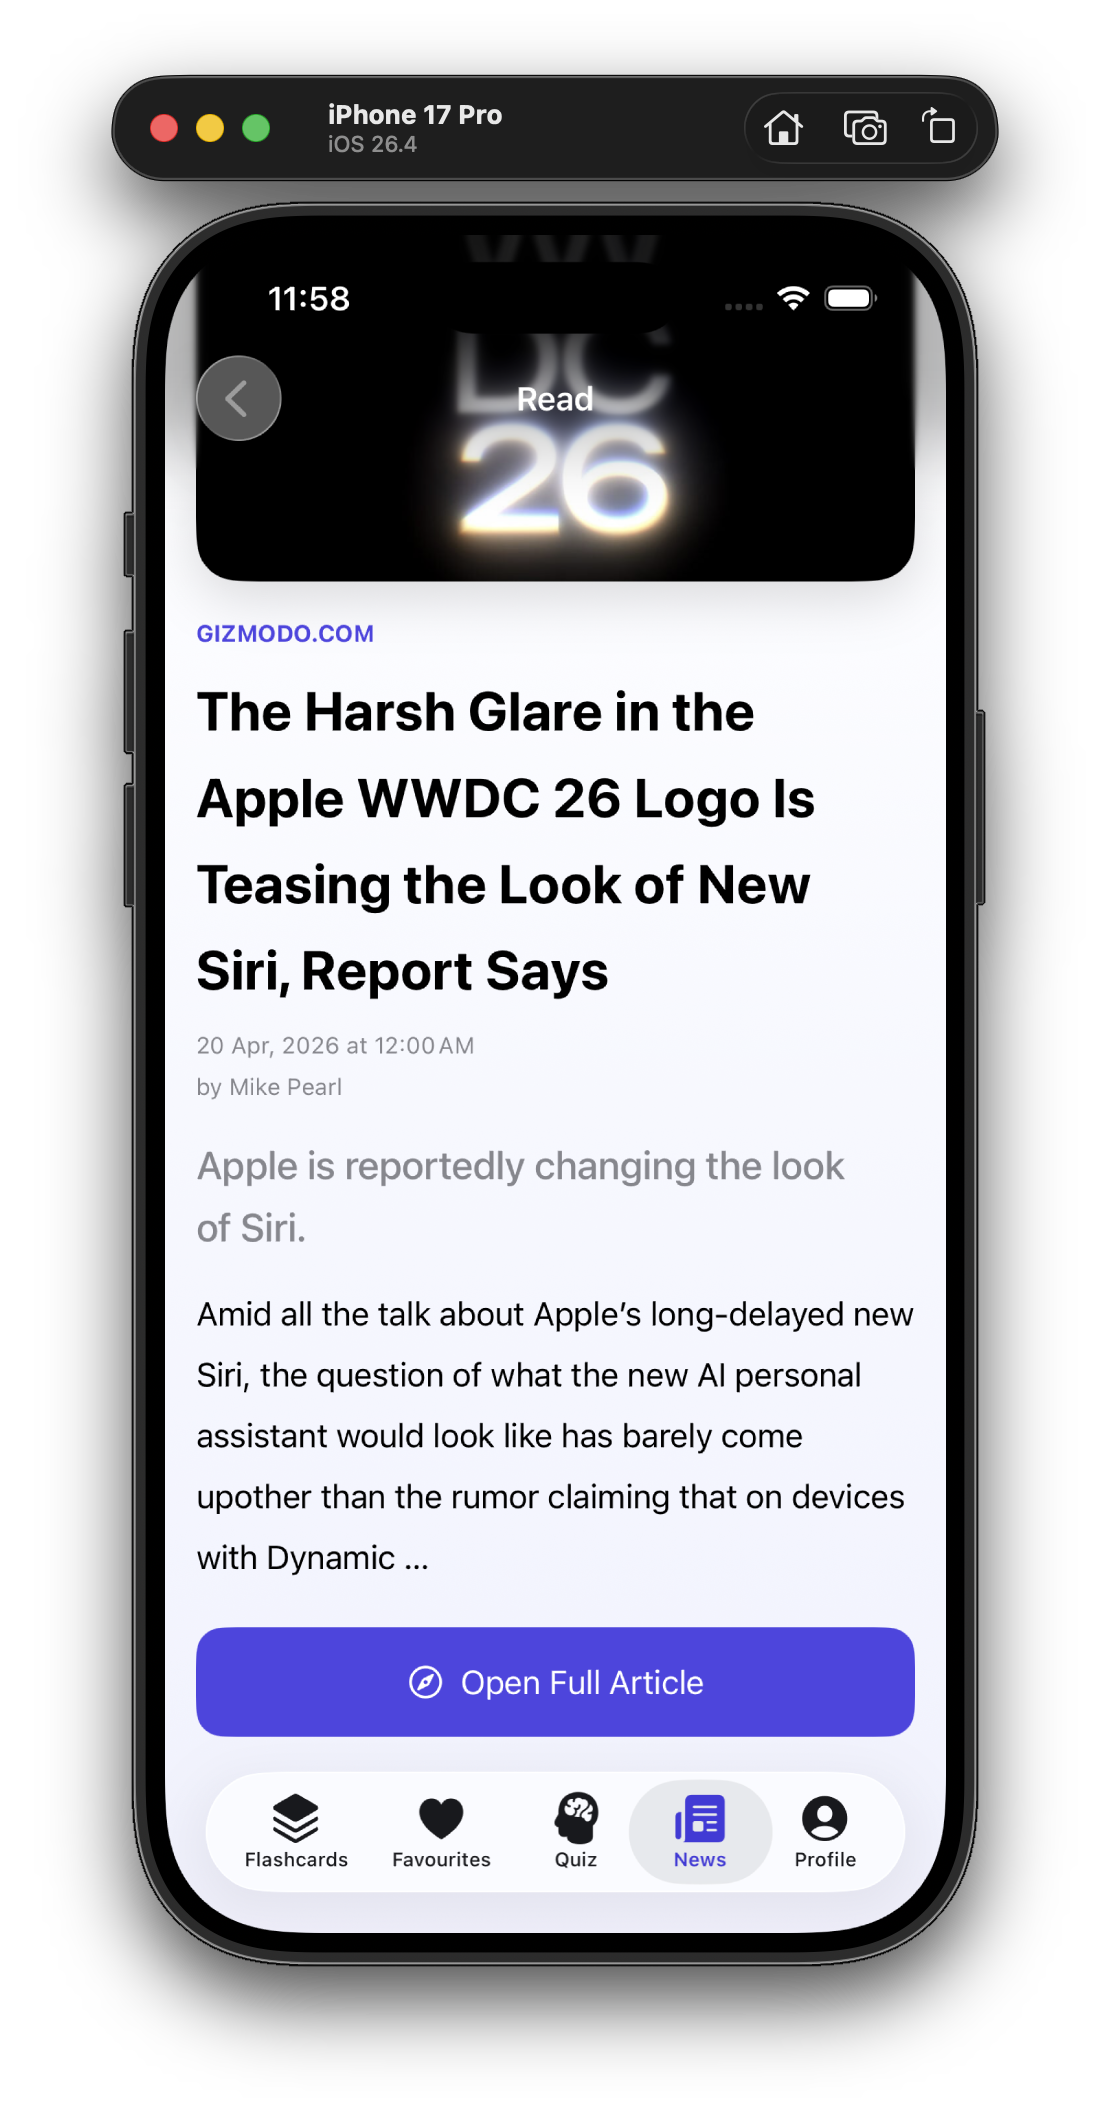
\includegraphics[width=0.30\textwidth]{SS/18. user_news_details_view_lower_part.png}\\[0.8em]
  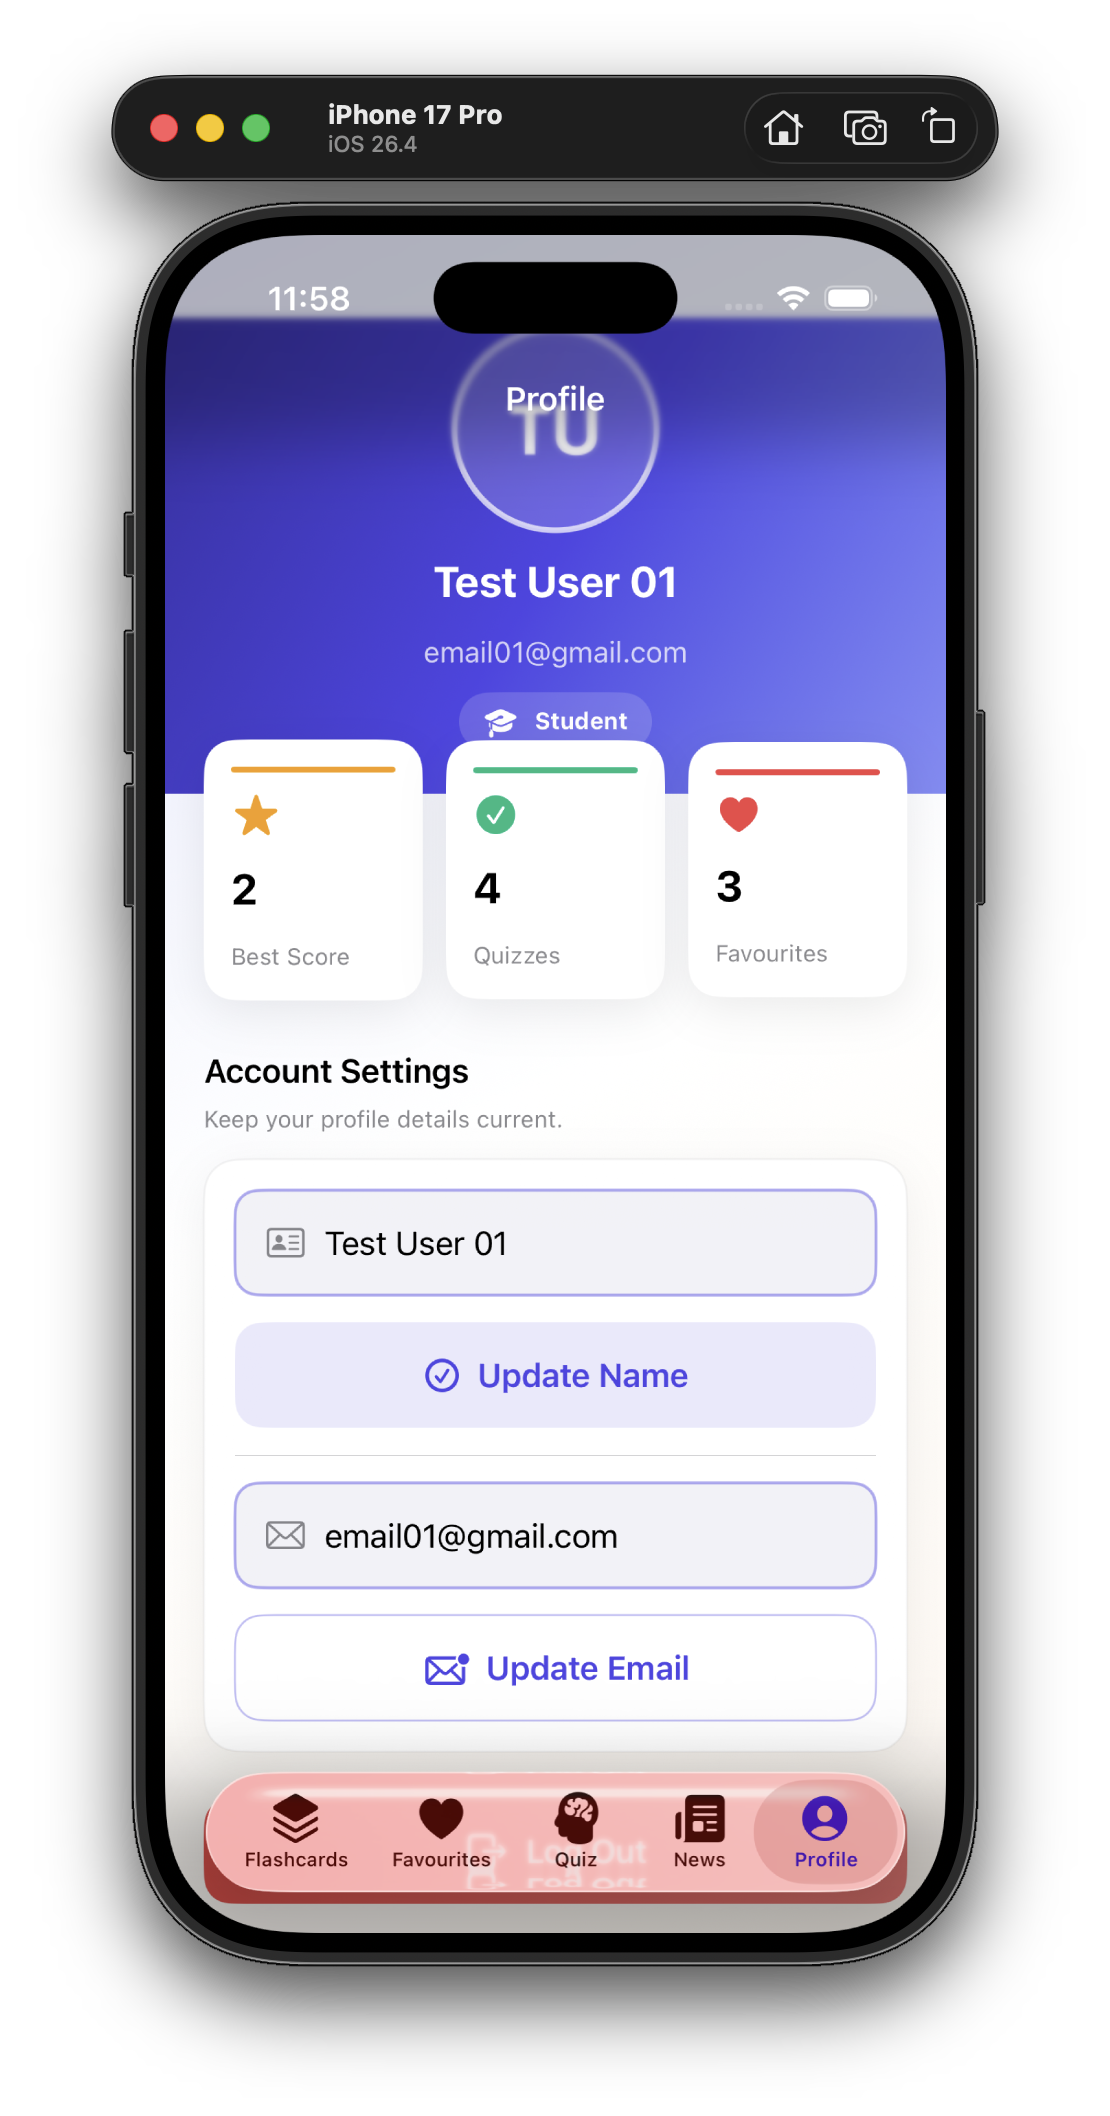
\includegraphics[width=0.30\textwidth]{SS/19. user_profile.png}\hfill
  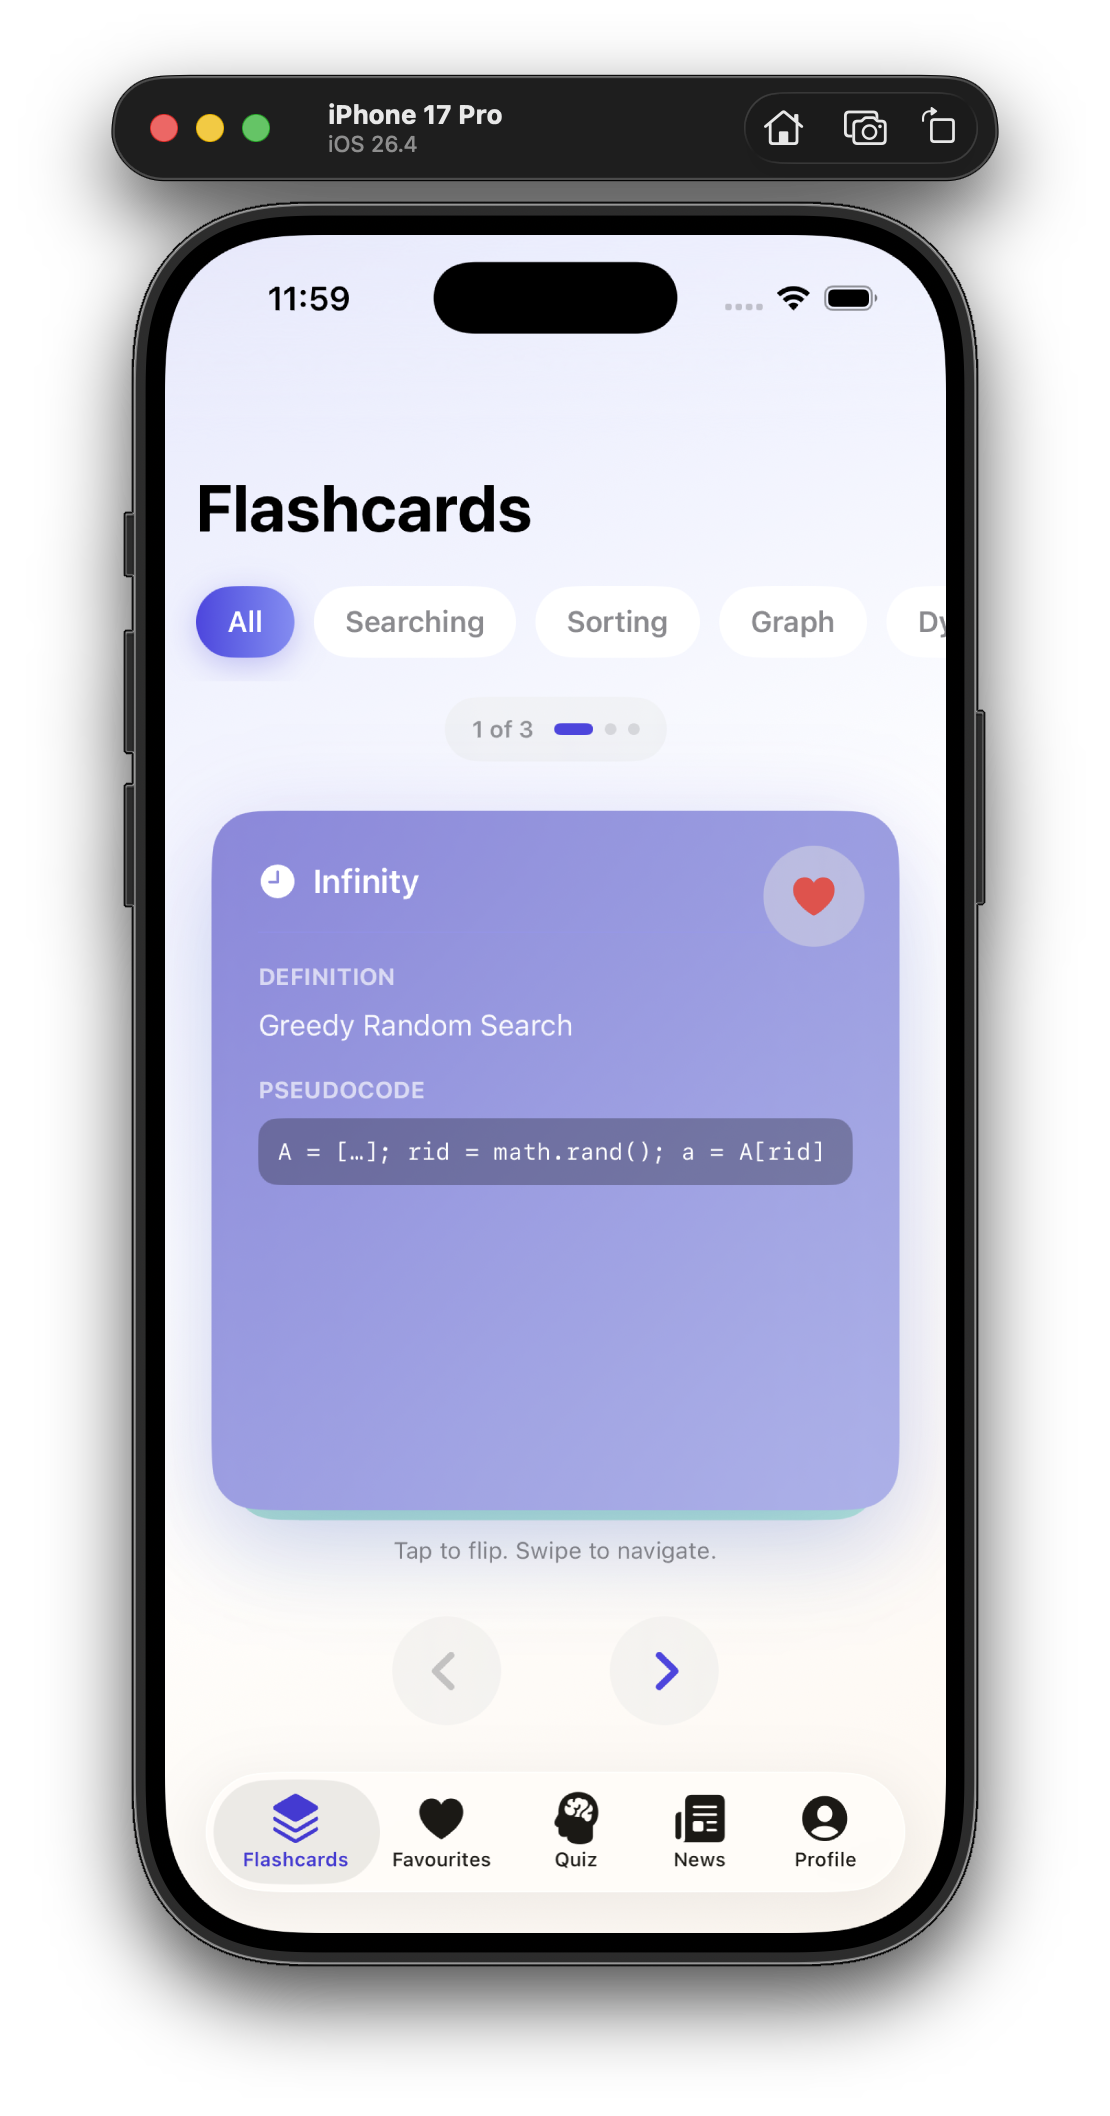
\includegraphics[width=0.30\textwidth]{SS/21. user_flashcard_flip_view.png}\hfill
  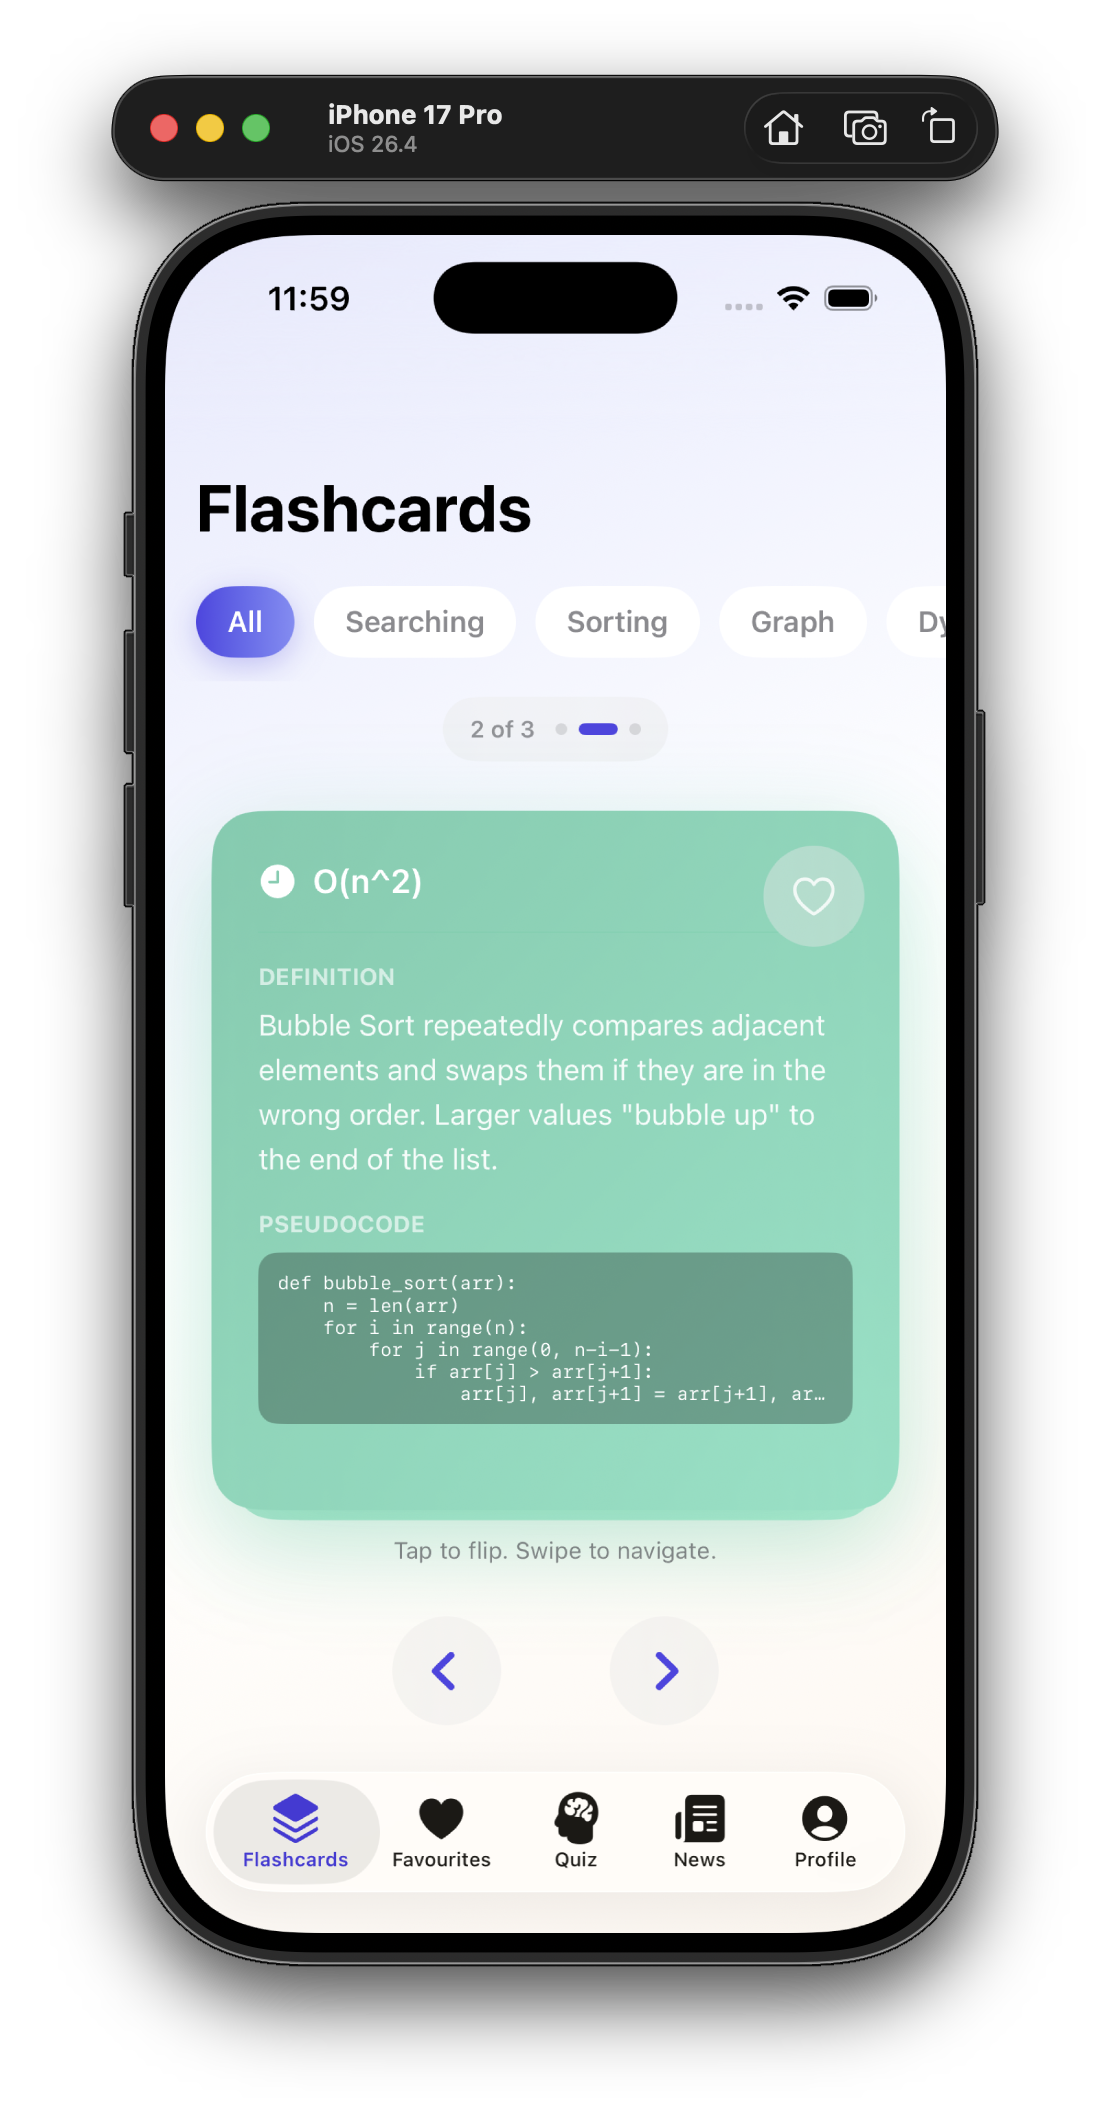
\includegraphics[width=0.30\textwidth]{SS/21. user_flashcard_flip_view_2.png}
  \caption*{Figure-6: Active Quiz Feedback, News, Profile Stats, and Flashcard Flip Views}
\end{figure}

% ══════════════════════════════════════════════════════════════════════════════
\section*{Team Contributions}
% ══════════════════════════════════════════════════════════════════════════════

\textbf{MD Ahsanul Islam:}\\
Authentication and Admin Dashboard --- Implemented Firebase Auth integration,
role-based routing in \texttt{ContentView}, and the full admin tab navigation
including flashcard and quiz management screens. Also Design Login and SignUp page layout.

\newpage
\medskip
\textbf{Md. Sabith:}\\
UI enhancement, Flashcards and Favourites --- Built the flashcard flip interaction, category filter
pills, difficulty badges, and the heart-toggle favourites system synced to Firestore. Enhance the User Interface and color combinations.

\medskip
\textbf{MD. Abu Hasanat Soykot:}\\
Quiz Mode, Profile and News --- Developed the timed quiz flow with immediate feedback,
score saving, and integrated the live NewsAPI feed with pull-to-refresh and
in-app Safari handoff. Also implement email and name updating method in the profile section for both the admin and the user. Also designed the result analytic tab in the admin side.
% ══════════════════════════════════════════════════════════════════════════════
\section*{Discussion}
% ══════════════════════════════════════════════════════════════════════════════

During development, one major challenge was managing role-based routing cleanly
without UI flicker. This was solved by keeping an unresolved role state in
\texttt{AuthViewModel} that shows a loading indicator until Firestore confirms the
user's role, before committing to either \texttt{MainTabView} or \texttt{AdminTabView}.

Another challenge was keeping the design consistent across two visually distinct
workspaces (user and admin). This was addressed by centralising all color tokens,
animations and reusable components in a single \texttt{DesignSystem.swift}
file, while using separate accent colors per workspace.

A third challenge was the live news integration: the NewsAPI key was initially
hardcoded in source, creating a security gap. The team flagged this as a known risk
and recommended moving it to an environment configuration file before any public
release.

Finally, synchronising profile edits across both Firebase Auth (display name/email)
and Firestore required careful sequencing in \texttt{ProfileViewModel} to avoid
partial updates when one service call succeeds and the other fails.

% ══════════════════════════════════════════════════════════════════════════════
\section*{Conclusion}
% ══════════════════════════════════════════════════════════════════════════════

AlgoFlash delivers a complete iOS algorithm learning experience built on SwiftUI and
Firebase. The app covers the full learning loop: study via interactive flashcards,
practice under timed quiz pressure, track personal progress, and stay current with
technology news. A shared design system ensures visual consistency across learner and
admin workspaces while keeping individual screens easy to extend.

Remaining work is concentrated in operational quality: restricting admin account
creation, moving API secrets out of source, adding automated test coverage, and
keeping documentation in sync with the codebase.

% ══════════════════════════════════════════════════════════════════════════════
\section*{References}
% ══════════════════════════════════════════════════════════════════════════════

\begin{itemize}[leftmargin=1.5em, itemsep=3pt]
  \item \url{https://developer.apple.com/documentation/swiftui}
  \item \url{https://developer.apple.com/documentation/combine}
  \item \url{https://firebase.google.com/docs/ios/setup}
  \item \url{https://firebase.google.com/docs/firestore}
  \item \url{https://newsapi.org/docs}
\end{itemize}

\end{document}